\documentclass[
    12pt, % Schriftgröße
    oneside, % zweiseitiger Modus
    ngerman, % deutsches Dokument
    BCOR=0mm, % Bindungskorrektur
    DIV=10 % Division (Anzahl Spalten/Zeilen pro Seite, bestimmt implizit Margins)
]{scrreprt}

\newcommand{\ArbeitTitelseite}{Dokumentation der Praktischen Arbeit\ zur Prüfung zum\ Mathematisch-technischen Softwareentwickler}
\newcommand{\titleDocument}{\ArbeitTitelseite}

\newcommand{\Autor}{Leonhard Aaron Keßler}
\newcommand{\authorDocument}{\Autor}

\newcommand{\ArbeitKopfzeile}{Dokumentation der Praktischen Arbeit 2022}
\newcommand{\ArbeitThema}{Bestimmung der Minimalanzahl von Antennen}
\newcommand{\Pruefungsnummer}{TODO}
\newcommand{\Programmiersprache}{Java}
\newcommand{\Compiler}{Maven}
\newcommand{\Rechner}{Dell Precision 7520}
\newcommand{\Betriebssystem}{Windows 10}


\newcommand{\subjectDocument}{Großprogrammierung}
\newcommand{\locationDocument}{Köln}
\newcommand{\dateDocument}{\today}

\title{\titleDocument}
\author{\authorDocument}
\date{\dateDocument}

%Style importieren:
\usepackage{dokumentation}


\begin{document}
    % ============ Anfang =============
    % Titelseite
    \begin{titlepage}
	% TODO: wird das geometry Paket genutzt statt der Mechanismen aus KOMA-Skript, kann die folgende Zeile z.B. durch "\newgeometry{...}" ersetzt werden
	\typearea{100} % DVI auf 100 setzen für Titel (kleine Margins)
	\setlength{\parindent}{0pt} % keine Einrückung bei neuen Absätzen auf dieser Seite

	\begin{flushright}
		\includegraphics[height=5cm]{images/FH-Aachen-r_svg-raw}
	\end{flushright}
	
	\vspace*{-2.5cm}

	\begin{center}
		\textbf{\Huge Fachhochschule~Aachen}

		\vspace*{0.5cm}
		
		\textbf{\Huge Studienort Köln}

		\vspace*{0.75cm}

		{\normalsize\doublespacing Fachbereich~9:~Medizintechnik~und~Technomathematik\\	Studiengang:~Angewandte~Mathematik~und~Informatik}

		\vspace*{2.5cm} % TODO: bei mehr verwendeten Zeilen für den Titel verringern
		
		\begin{minipage}[t]{16cm} % TODO: abhängig von dem konkreten Titel muss diese Breite eventuell angepasst werden für einen passenden Zeilenumbruch
			\begin{center}
				\textbf{\Huge \titleDocument}
			\end{center}
		\end{minipage}
	
		\vspace*{2cm} % TODO: bei mehr verwendeten Zeilen für den Titel verringern (symmetrisch zu oben)
		
		\textbf{\Large \subjectDocument}

		\vspace*{0.5cm}
		
		{\normalsize von}
		
		\vspace*{0.5cm}
		
		\textbf{\Large \authorDocument}
	
		\vspace*{3.5cm}
		
		\begin{minipage}[t]{13cm}
			\begin{center}
				\begin{tabular}{ll}
					Matrikelnummern: & 3235914 \\
				\end{tabular}
			\end{center}
		\end{minipage}
		
		\vspace*{2.5cm}
	
		{\large \locationDocument, den \dateDocument}
	\end{center}
\end{titlepage}


    \tableofcontents

    % =========== Zahlenteil ===========
    \chapter{Aufgabenanalyse}\label{ch:aufgabenanalyse}
\section{Interpretation der Aufgabe}\label{sec:interpretation-der-aufgabe}
\subsection{Sachverhalt}\label{subsec:sachverhalt}
Der Sachverhalt der Aufgabenstellung handelt von einem Bahnnetz. Dieses beinhaltet mehere Bahnstationen die Teil einer oder meherer Zugverbindungen sein können. Der Sachverhalt setzt vorraus, dass Züge bei jeder Fahrt an Servicestationen versorgt werden müssen.
\subsection{Problemstellug}\label{subsec:aufgabenstellung}
Gefordert ist ein Programm, welches die Positionen von Servicestationen ermittelt. Dafür muss gelten, dass jede Zugverbindung des angegebenen Bahnnetz mindestens eine Servicestation beinhaltet. In der Folge sollen Bahnstationen ermittelt werden die für das Bahnnetz als Servicestationen dienen können und somit alle Zugverbindungen des Bahnnetzes abdecken. Die Anzahl der Servicestationen soll dabei so gering wie möglich sein.
\\
Um die Speicherkapazitäten zu minimieren und die Programmlaufzeit zu optimieren werden zusätzliche Reduktionsverfahren auf die Zugverbindungensdaten angewendet werden.\\ 

\section{Präzisierung der Teilaufgaben}\label{subsec:teilaufgaben}
\subsection{Eingabe}\label{subsec:eingabe}
Die Umsetzung erfolgt auf Basis eines Bahnnetzes, welches aus einer Datei eingelesen werden kann. Die Dateiendung ist dabei frei wählbar. Aus dieser Datei können die verschiedenen Zugverbindungen eingelesen werden. Diese bilden das Bahnnetz ab.\\
Beginnt eine Zeile mit einem \enquote{\#} so wird diese als Kommentar interpretiert. Einzelne Zugverbindungen werden mit Zeilenumbrüchen getrennt. Die darin enthaltenden Bahnstationen sind durch Semikolons seperierbar.\\

\subsection{Datenreduktion}\label{subsubsec:datenreduktion}
Auf diese Bahnstationen werden nun drei verschiedene Reduktionsverfahren angewendet. Diese sollen die Anzahl der Bahnstationen und Bahnverbindungen reduzieren, ohne dabei einen Informationsverlust zu riskieren.\\ 

\subsubsection{Doppelstationen}\label{subsubsec:doppelstationen}
Doppelte Stationen innerhalb einer Zugverbindung werden entfernt.

\subsubsection{Stationsabhängigkeiten}\label{subsubsec:stationsabhaengigkeiten}
Voneinander abhängige Stationen werden zusammengefasst.

\subsubsection{Implizite Zugverbindungen}\label{subsubsec:implizite-zugverbindungen}
Zugverbindungen die andere Zugverbindungen beinhalten, werden entfernt.
\\
\subsection{Algorithmus}\label{subsec:algorithmus}
Zur Berechnung des Algorithmus werden die übergebliebenen Bahnstationen gesammelt. Anhand derer wird nun die minimale Anzahl an Servicestationen ermittelt. Der dafür zuständige Algorithmus ist ein iteratives Vorgehen, welches nach Greedy-Prinzipien arbeitet.\\
\\
\subsection{Ausgabe}\label{subsec:ausgabe}
Im Anschluss an die Berechnung wird die Ausgabe erzeugt. Diese besteht aus einer einzeiligen .txt Datei. In dieser werden, identisch zur Eingabedatei, die ermittelten Bahnstationen semikolongetrennt aufgelistet.\\

\begin{figure}[h]
    \centering
    \caption{Input-Restriktionen}
    \begin{itemize}[noitemsep]
        \item Es muss mindestens eine (nicht Kommentar-) Zeile vorhanden sein
        \item Jede Zeile muss mindestens 2 Stationen enthalten
        \item Jede Zeile darf beliebig viele Stationen enthalten
        \item Es dürfen beliebig viele Zeilen vorhanden sein
        \item Es dürfen beliebig viele Kommentar-Zeilen vorhanden sein
        \item Semikolons dürfen nicht am Anfang oder Ende einer Zeile stehen
        \item Semikolons dürfen nicht hintereinander stehen
    \end{itemize}
    \label{fig:input-restrictions}
\end{figure}

\begin{figure}[h]
    \centering
    \caption{Stationnamen-Restriktionen}
    \begin{itemize}[noitemsep]
        \item Ein Name darf nur aus Buchstaben von A bis Z bestehen
        \item Ein Name darf aus maximal 3 Buchstaben bestehen
    \end{itemize}
    \label{fig:stationname-restrictions}
\end{figure}


\section{Fehlerarten}\label{sec:fehlerarten}
Die Eingabedatei kann verschiedene Integritätsbedingungen verletzen.
Das Programm muss diese Fehlerarten identifizieren und den Nutzer darüber informieren.

\subsection{Technische Fehler}\label{subsec:technische-fehler}
Technische Fehler entstehen, wenn dem Programm ein nicht existierender Dateiname übergeben wird.

\subsection{Syntaktische Fehler}\label{subsec:syntaktische-fehler}
Die Eingabedatei muss der Struktur aus~\nameref{fig:input-restrictions} entsprechen.
So kann zum Beispiel ein syntaktischer Fehler provoziert werden, indem Stationnamen nicht semikolongetrennt sind.

\subsection{Semantische Fehler}\label{subsec:semantische-fehler}
Die eingelesenen Stationnamen müssen der Struktur aus~\nameref{fig:stationname-restrictions} entsprechen.
So kann zum Beispiel ein syntaktischer Fehler provoziert werden, indem Stationnamen Zahlen beinhalten.

\section{Fehlerbehandlung}\label{sec:fehlerbehandlung}

\subsection{Technische Fehler}\label{subsec:technische-fehler-behandlung}
Ist ein technischer Fehler vorhanden, wird eine Ausnahme geworfen und das Programm beendet.


\subsection{Syntaktische Fehler}\label{subsec:syntaktische-fehler-behandlung}
Wird ein syntaktischer Fehler identifiziert, wird eine Ausnahme geworfen und das Programm beendet. Außerdem wird eine Erklärung für die korrekte Syntax der Eingabedatei ausgegeben.

\subsection{Semantische Fehler}\label{subsec:semantische-fehler-behandlung}
Wird ein syntaktischer Fehler identifiziert, wird eine Ausnahme geworfen und das Programm beendet. Außerdem wird eine Erklärung für gültige Stationnamen ausgegeben.


\subsection{Sonderfälle}\label{subsec:sonderfaelle}
Nach der Datenreduktion kann es sein, dass eine Zugverbindung nurnoch aus einer Station besteht. Beim einlesen von Zugverbindungen ist dies ungültig und wirft eine Ausnahme. Nach dem Einlesen und somit auch nach der Datenreduktion ist dies jedoch wieder erlaubt und ist eine gültige Zugverbindung.\\

    \chapter{Verfahrensbeschreibung}\label{ch:verfahrensbeschreibung}


\section{Gesamtsystem}\label{ver:sec:gesamtsystem}
Das System arbeitet nach dem EVA-Prinzpip. Die EVA-Segmente werden von einem Controller erweitert, welcher das Programm koordiniert und den Einstiegspunkt des Programms darstellt.

\subsection{Eingabe}\label{ver:subsec:eingabe}
Um ein vollständiges Bahnnetz abbilden zu können werden alle Bahnverbindungen aus der Eingabedatei eingelesen. Dafür werden die einzelnen Stationen einer Verbindung als \texttt{String} in eine \texttt{ArrayListe} gespeichert. Diese Listen lassen sich dann in ein Objekt Objekt Zugverbindung (siehe \ref{ver:subsubsec:trainconnection}) umwandeln. Die erstellten \texttt{TrainConnection}-Objekte werden in einer Liste gesammelt und nach einlesen der Datei dem Controller übergeben.\\

\subsection{Verarbeitung}\label{subsec:verarbeitung}
Die Liste mit den Zugverbindungen kann nun weiterverarbeitet werden. Dafür wird diese in ein Objekt \texttt{TrainWeb}(\ref{ver:subsubsec:trainweb}) umgewandelt welches Hauptbestandteil der Datenspeicherung ist.\\
Vor der eigentlichen Berechnung des Algorithmus wird das Netzt nun noch reduziert. Dafür wird dieses einem \texttt{Reducer}(\ref{ver:subsubsec:reducer}) übergeben, der die Verbindungen und die darin enthaltenen Staionen in eine minimale aber informationsidentische Form reduziert. \\
Nach der Reduktion wird das reduzierte Netz an den Algorithmus übergeben. Dieser ermittelt nun die minimale Anzahl an Servicestationen und deren Standorte. Die Standorte werden als \texttt{Station}(\ref{ver:subsubsec:station}) in einer \texttt{ArrayList} zurück an den Controller übergeben\\

\subsection{Ausgabe}\label{ver:subsec:ausgabe}
Die ermittelte Liste wird nun an die Ausgabe weitergegeben. Diese nimmt die Liste mit den ermittelten Stationen entgegen und schreibt diese in eine Ausgabedatei.\\

\section{Datenstrukturen}\label{ver:subsec:datenstrukturen}
Um die Verarbeitung der Daten übersichtlich zu gestalten werden verschiedene Datenstrukturen erstellt. Dabei lässt sich unterscheiden in Speicher Strukturen und Verarbeitungsstrukturen.\\
\subsection{Speicherstrukturen}\label{ver:subsec:Speicherstrukturen}
Alle erstellten Datenstrukturen basieren auf ArrayListen. Diese bieten einerseits eine dynamische Speichermöglichkeit. Andererseits ermöglicht dies ein optimale Speicherung, da durch die Nutzung von ArrayListen die Zugnetzdaten nur einmal gespeichert und dann als Referenzen weitergegeben werden können. Dies verhindert unnötiges Kopieren und erleichtert Vergleiche.\\

\subsubsection{TrainConnection}\label{ver:subsubsec:trainconnection}
Hauptbestandteil der Datenvermittlung ist die Klasse \texttt{TrainConnection}. Diese besitzt als einziges Attribut eine \texttt{ArrayList} in welcher Stationen als String abgespeichert werden. Diese Stationen bilden dann eine vollständige  Zugverbindung ab.

Außerdem sind zwei Vergleichmethoden implementiert. Diese ermöglichen die gespeicherte Liste an Stationen, von zwei Objekten TrainConnection
 miteinander zu vergleichen. Eine Methode vergleicht die Anzahl der Stationen (hat die Verbindung mehr Haltestellen als die andere?). Die zweite Methode überprüft den Inhalt der Stationen (fahren beide Verbindungen die gleichen Stationen an?)\\

\subsubsection{Station}\label{ver:subsubsec:station}
Um im Verlaufe der Verfahren strukturiert vorgehen zu können existiert die Klasse \texttt{Station}. Diese speichert den Namen einer Station als \texttt{String} und eine \texttt{ArrayListe} mit Bahnverbindungen(\ref{ver:subsubsec:trainconnection}) in der der die Station angefahren wird.\\
Wie in \ref{ver:fig:datenstruktur_zusammenhaenge} zu sehen, werden dabei keine Kopien der \texttt{TrainConnection}'s erstellt sondern nur Referenzen auf die ursprünglichen Objekte gespeichert.\\
Diese Klasse ist dabei nur eine Hilfestellung für spätere Operationen. Die eigentlichen Bahnstationen werden weiterhin als \texttt{String} gespeichert und verglichen. Durch diese Klasse wird verhindert, jedesmal alle Bahnverbindungen zu ermitteln zu müssen in denen eine Station vorkommt.\\

\subsubsection{TrainWeb}\label{ver:subsubsec:trainweb}
Mit diesen beiden Speicherstrukturen lässt sich nun das gesamte Bahnnetz übersichtlich speichern. Dafür stehen in dem Objekt \texttt{TrainWeb} zwei Attribute zur Verfügung. Eine \texttt{ArrayListe} mit allen Bahnverbindungen(\ref{ver:subsubsec:trainconnection}) und eine \texttt{ArrayListe} mit allen Bahnstationen(\ref{ver:subsubsec:station}).
Dafür werden alle Verbindungen aus der eingelesen Datei direkt abgelegt. Die Bahnstationen können nun über das Iterieren aller Bahnverbindungen ermittelt werden. Für neue Stationen wird dann erneut über alle Verbindungen iteriert, um alle stationsbeinhaltende Verbindungen zusammen mit dem Stationsnamen als \texttt{Station}-Objekt (\ref{ver:subsubsec:station}) speichern zu können.\\

\begin{center}
    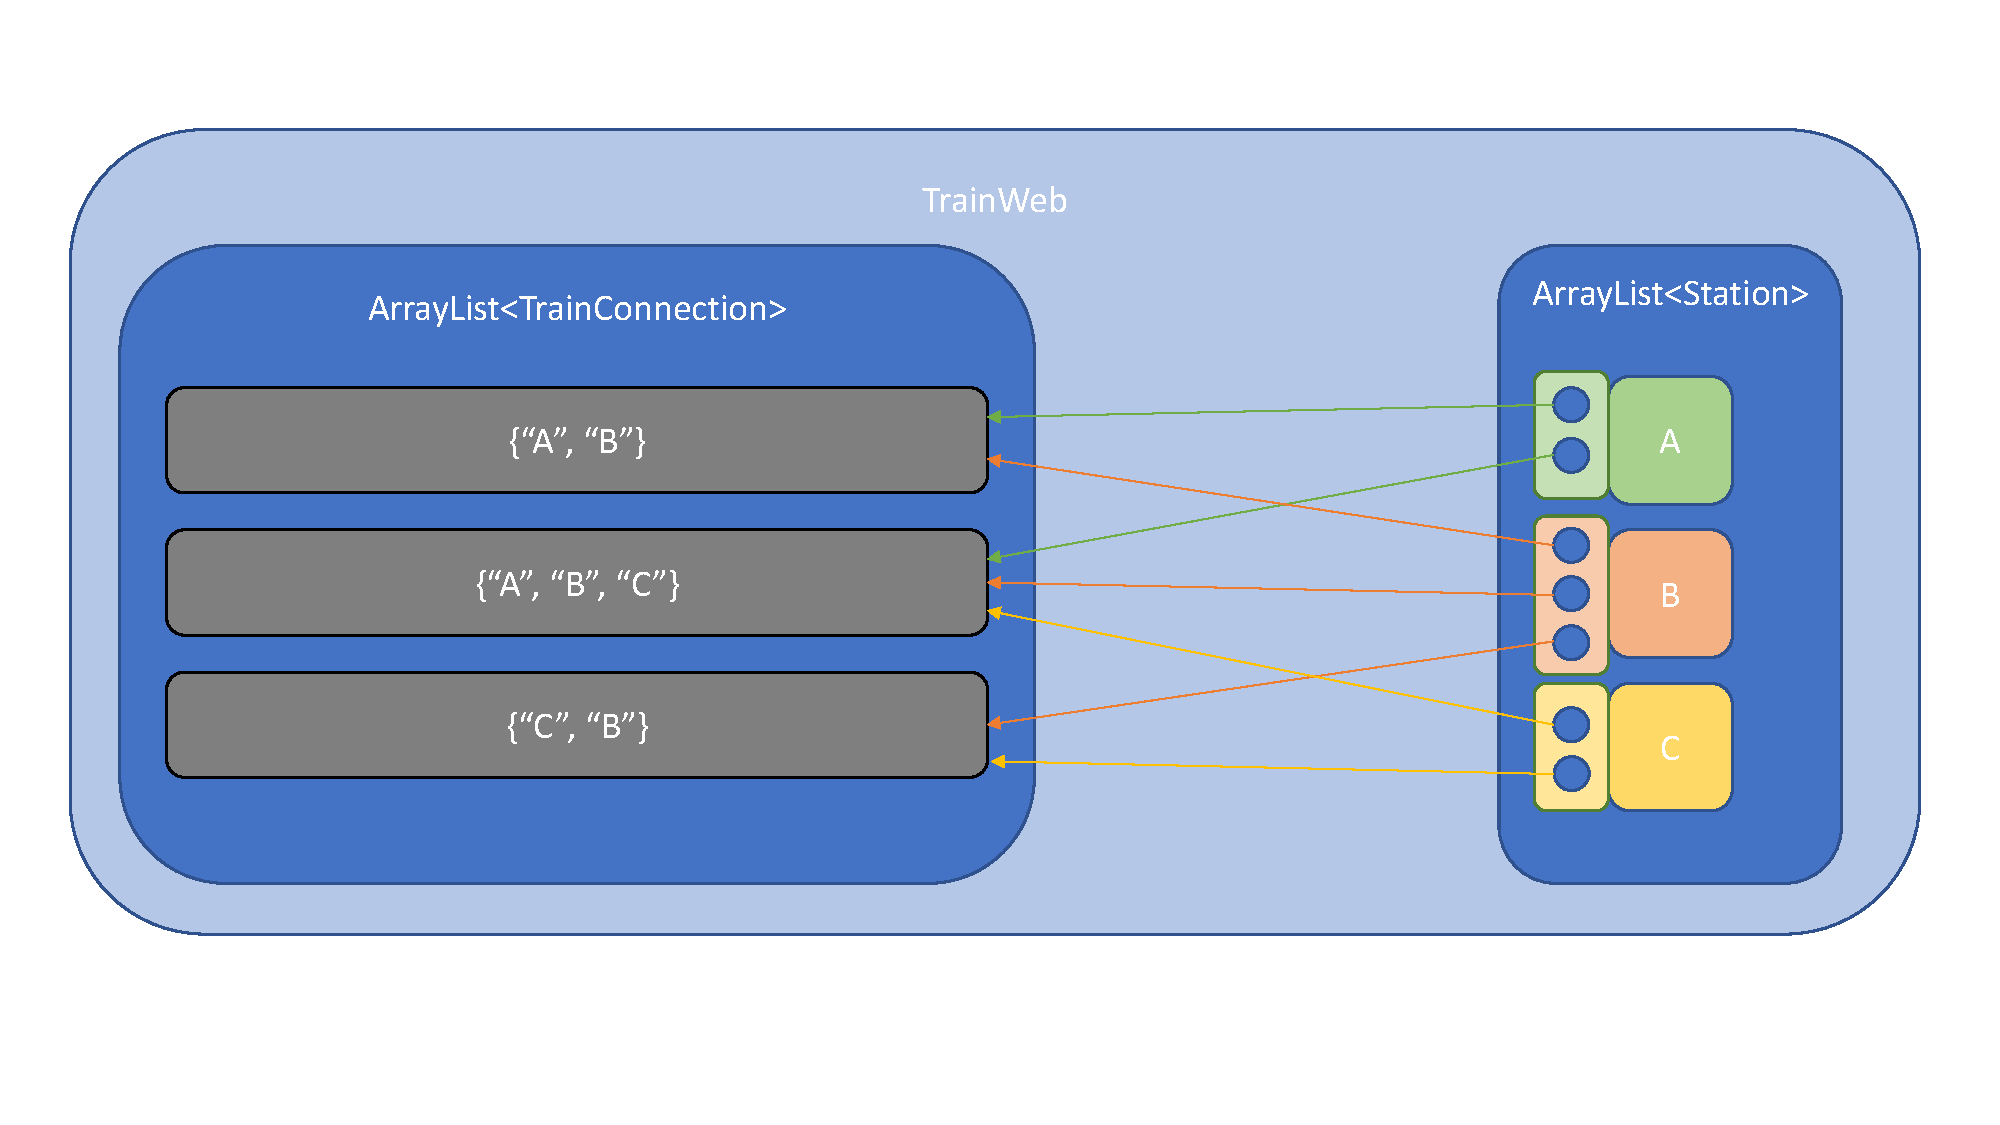
\includegraphics[width=\linewidth]{images/Datenstruktur_Zusammenhaenge.pdf}
    \captionof{figure}{Speicherstrukturen und ihre Zusammenhänge}
    \label{ver:fig:datenstruktur_zusammenhaenge}
\end{center}

\subsection{Verarbeitungsstrukturen}\label{ver:subsec:verarbeitungsstrukturen}
Die Verarbeitungsstrukturen nehmen nun einen fertigen Netzplan entgegen auf dem sie arbeiten.\\

\subsubsection{Reducer}\label{ver:subsubsec:reducer}
Der Reducer hat dabei keinen Rückgabewert. Dieser wendet die drei, als Methoden implementierten, Reduktionsverfahren(siehe \ref{ver:subsec:reduktionsverfahren}) direkt auf den Netzplan an.\\

\subsubsection{Algorithmus}\label{ver:subsubsec:algorithmus}
Der reduzierte Netzplan wird nun dem Algorithmus übergeben. Dieser ermittelt anhand des Plans, Bahnstationen um das gesamte Netz versorgen zu können.

\section{Verbale Beschreibung der Verfahren}\label{ver:sec:verfahren}
Um sicher zu gehen, ob es sich um die minimale Lösung handelt läuft nun ein Prozess der die aktuell gefundenen Bahnstationen überprüft. Sollte eine Bahnstation keinen Einfluss auf die erreichbaren Verbindungen haben wird dieser entfernt. Wenn dies auf mehere Bahnhöfe zutrifft wird der Bahnhof gelöscht, der mehr Verbindungen abgedeckt.\\

\subsection{Reduktionsverfahren}\label{ver:subsec:reduktionsverfahren}
\subsubsection{Doppelstationen}\label{ver:subsubsec:doppelstationen}
In diesem Verfahren werden alle Zugverbindungen nach Mehrfachvorkommen von Stationen geprüft. Sollte eine Station mehrfach in einer Verbindung angefahren werden, braucht diese nur einmal in der Zugverbindung gespeichert werden. Für die spätere Berechnung ist nur relevant welche Stationen in einer Zugverbindung angefahren werden. Die Reihenfolge der Stationen spielt somit keine Rolle. Somit gehen durch die einfache Speicherung von Stationen keine Inforamtionen verloren.\\

\subsubsection{Stationsabhängigkeiten}
In diesem Verfahren werden Stationsabhängigkeiten geprüft. Sollte in allen Zugverbindung die eine beliebige Station A beinhaltet, auch eine Station B angefahren werden kann die betrachtete Station A in allen Zugverbindungen entfernt werden. Es ist davon auszugehen, dass dabei kein Informationsverlust riskiert wird, da jede Zugverbindung der betrachteten Station A auch die gefundene Station B passieren wird. Die Menge der Zugverbindungen die Station A anfahren ist also eine Teilmenge der Verbindungen Station B und müssen nichtmehr gesondert gespeichert und überprüft werden. Dabei kann es dazu kommen, dass Zugverbindungen aus nurnoch einer Station bestehen.\\

\subsubsection{Implizite Zugverbindungen}
In diesem Verfahren wird überprüft ob eine Zugverbindung implizit in einer anderen Zugverbindung enthalten ist. Sollte dies der Fall sein, darf die größere Zugverbindung entfernt werden. Dies ist erlaubt, da alle Stationen der kleineren Verbindung auch in der größeren Verbindung angefahren werden. Eine Überprüfung der kleineren Zugverbindung ist also Ausreichend um beiden Verbindungen eine Servicestationen zu gewährleisten. Die größere Verbindung ist somit redundant.\\

\subsection{Berechnung der minimalen Anzahl an Servicestationen}\label{ver:subsec:berechnung}
Der Algorihtmus wählt aus den Stationen des Netzplans, die Station aus, die in den meisten Verbindungen auftaucht. Diese wird in einer Liste gespeichert. Daraufhin startet eine Schleife, die solange Bahnhöfe der Liste hinzufügt, bis alle Verbindungen versorgt werden. Dabei werden immer die Bahnhöfe ausgewählt, die in den noch nicht versorgten Verbindungen die meisten neuen Zugverbindungen versorgen können.\\

    \chapter{Programmbeschreibung}\label{pro:ch:programmbeschreibung}

\section{Struktogramme}\label{pro:sec:pap}

\subsection{UML-Klassendiagramm}\label{pro:subsec:uml-klassendiagramm}
\begin{center}
    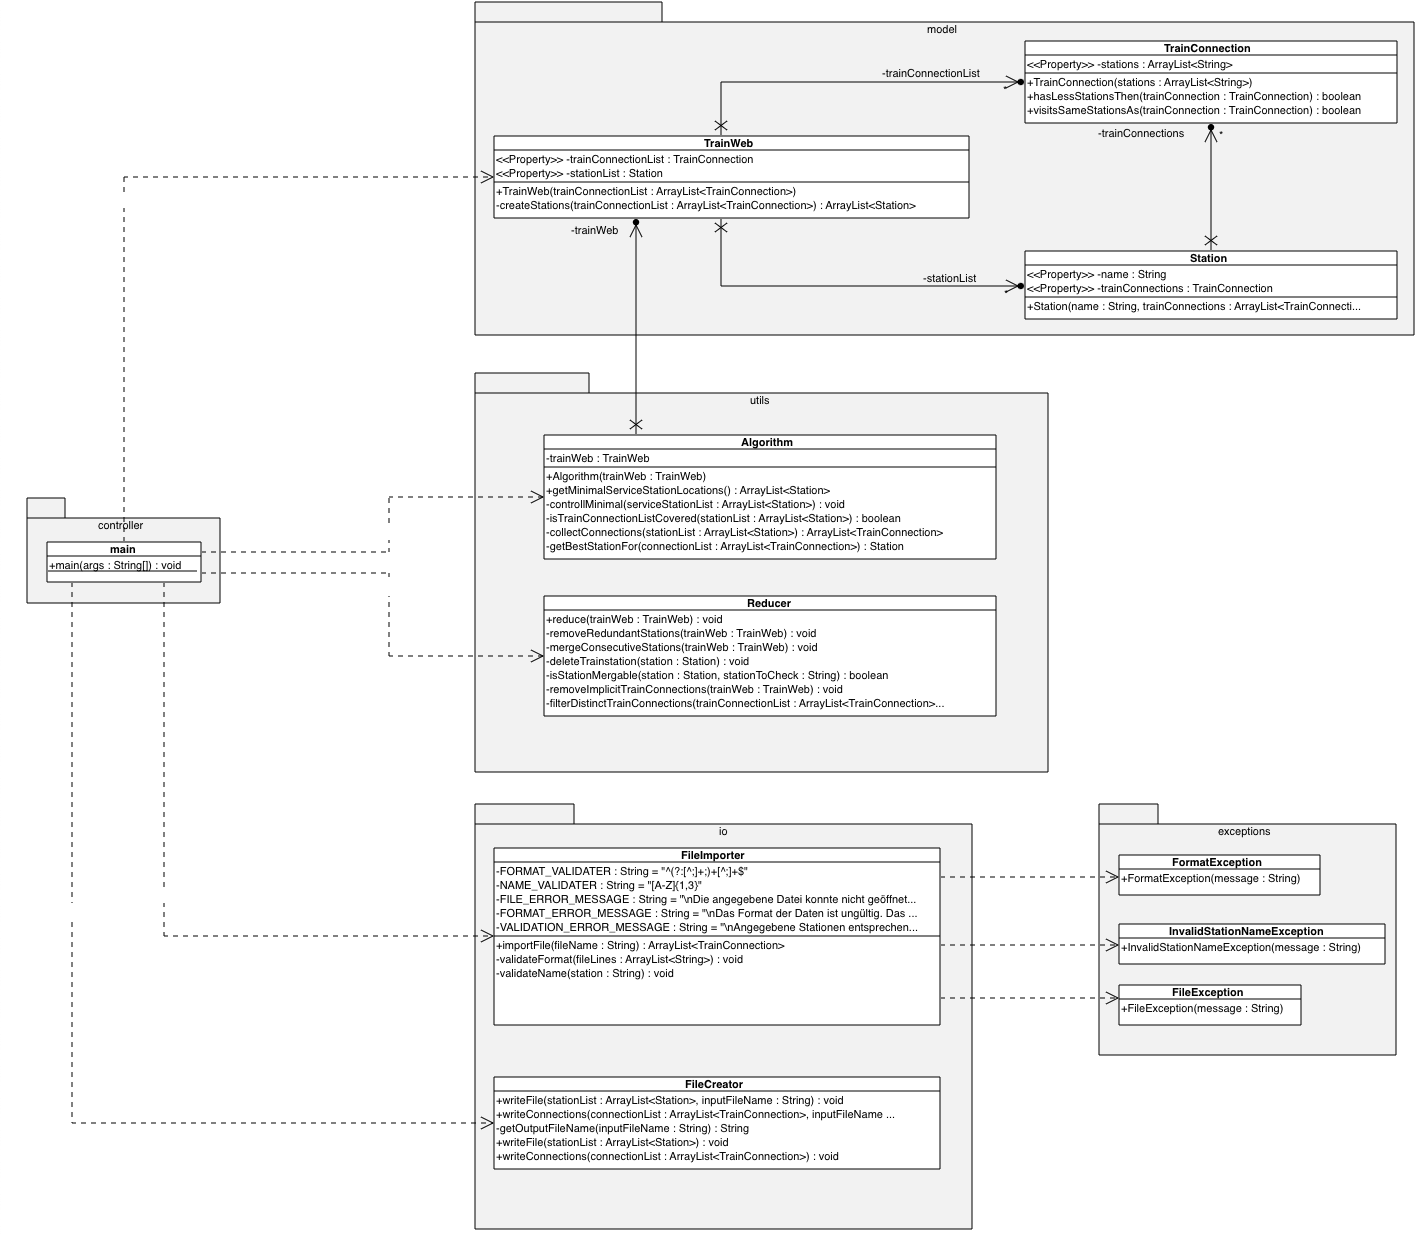
\includegraphics[width=\linewidth]{images/Struktogramme/UML-Klassendiagramm.png}
    \captionof{figure}{UML-Klassendiagramm}
    \label{pro:subsecpar:uml-klassendiagramm}
\end{center}

\subsection{UML-Sequenzdiagramm}\label{pro:subsec:uml-sequenzdiagramm}
\begin{center}
    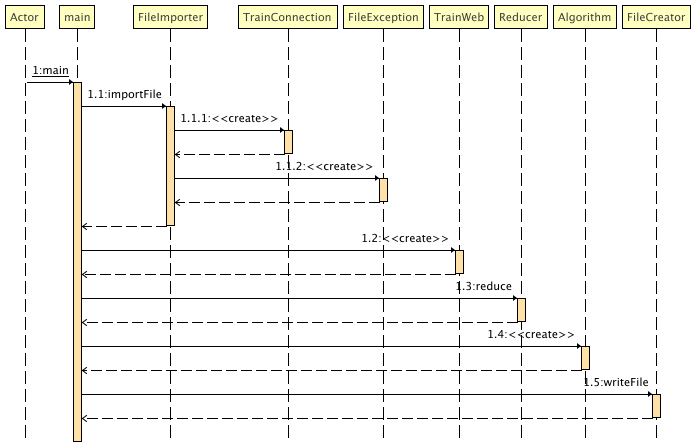
\includegraphics[width=\linewidth]{images/Struktogramme/Sequenzdiagramm.png}
    \captionof{figure}{UML-Sequenzdiagramm}
    \label{pro:subsecpar:uml-sequenzdiagramm}
\end{center}

\newpage
\subsection{Nassi-Shneiderman-Diagramme}\label{pro:subsec:nassi-shneiderman-diagramme}
\subsubsection{Input / Output}\label{pro:subsubsec:io}
\paragraph{Input}\label{pro:subsubsecpar:input}
\begin{center}
    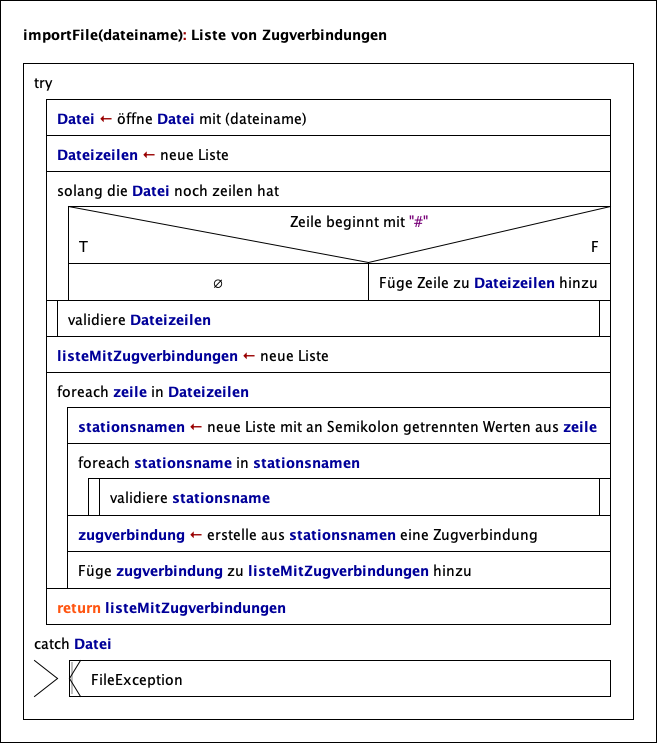
\includegraphics[width=\linewidth]{images/Struktogramme/io/importFile.png}
    \captionof{figure}{Input}
    \label{pro:subsubsecpar:inputFile}
\end{center}

\begin{center}
    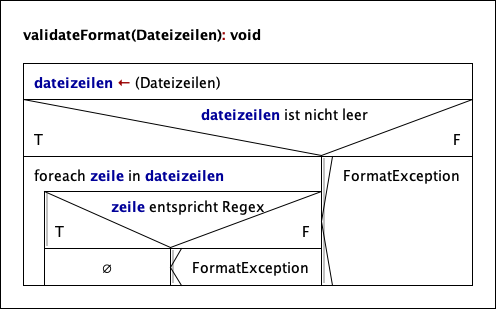
\includegraphics[width=\linewidth]{images/Struktogramme/io/validateFormat.png}
    \captionof{figure}{Format Validator}
    \label{pro:subsubsecpar:format-validator}
\end{center}

\begin{center}
    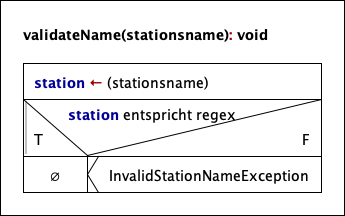
\includegraphics[width=\linewidth]{images/Struktogramme/io/validateName.png}
    \captionof{figure}{Namen Validator}
    \label{pro:subsubsecpar:namen-validator}
\end{center}


\paragraph{Output}\label{pro:subsubsecpar:output}
\begin{center}
    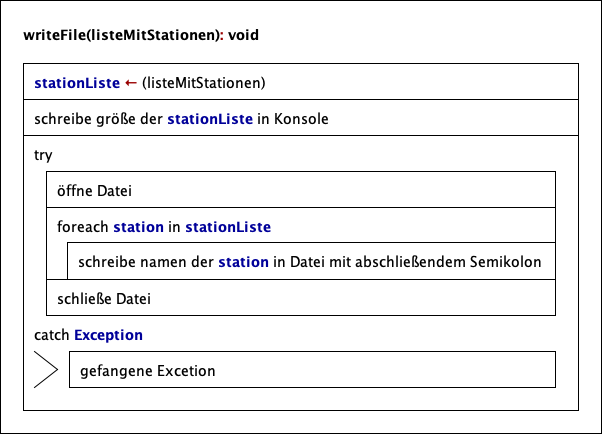
\includegraphics[width=\linewidth]{images/Struktogramme/io/writeFile.png}
    \captionof{figure}{Namen Validator}
    \label{pro:subsubsecpar:namen-validator}
\end{center}


\newpage
\subsubsection{Reduzieren}\label{pro:subsubsec:reduzieren}
\paragraph{Doppelstationen}\label{pro:subsubsubsec:doppelstationen}
\begin{center}
    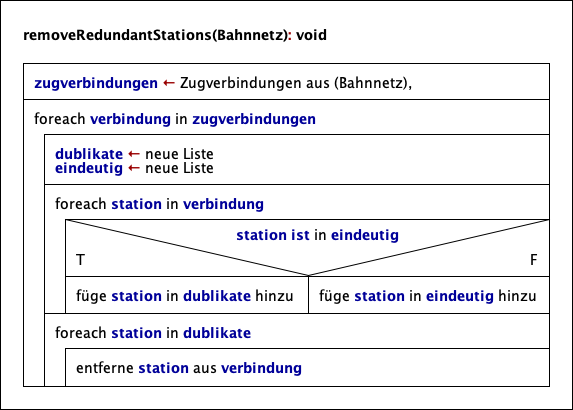
\includegraphics[width=\linewidth]{images/Struktogramme/reducer/reduction1/removeRedundantStations.png}
    \captionof{figure}{Entfernen von Doppelstationen}
    \label{pro:subsubsecpar:entfernen-von-doppelstationen}
\end{center}


\paragraph{Stationsabhängigkeiten}\label{pro:subsubsubsec:stationsabhaengigkeiten}
\begin{center}
    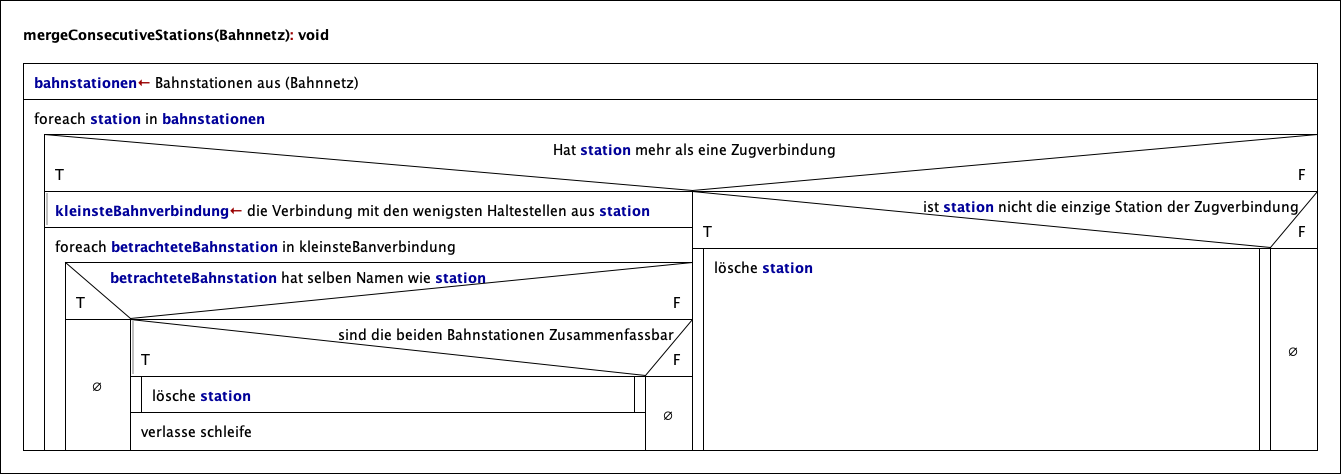
\includegraphics[width=\linewidth]{images/Struktogramme/reducer/reduction2/mergeConsecutiveStations.png}
    \captionof{figure}{Zusammenfassen von Stationen}
    \label{pro:subsubsecpar:zusammenfassen-von-stationen}
\end{center}

\begin{center}
    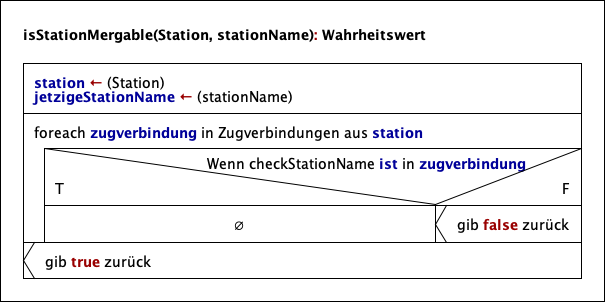
\includegraphics[width=\linewidth]{images/Struktogramme/reducer/reduction2/isStationMergable.png}
    \captionof{figure}{Überprüfung ob Stationen zusammenfassbar sind}
    \label{pro:subsubsecpar:ueberpruefung-ob-stationen-zusammenfassbar-sind}
\end{center}

\begin{center}
    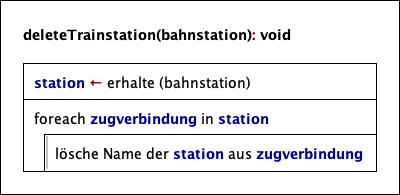
\includegraphics[width=\linewidth]{images/Struktogramme/reducer/reduction2/deleteTrainstation.png}
    \captionof{figure}{Entfernen von Stationen}
    \label{pro:subsubsecpar:entfernen-von-stationen}
\end{center}


\paragraph{Implizite Zugverbindungen}\label{pro:subsubsubsec:implizite-zugverbindungen}
\begin{center}
    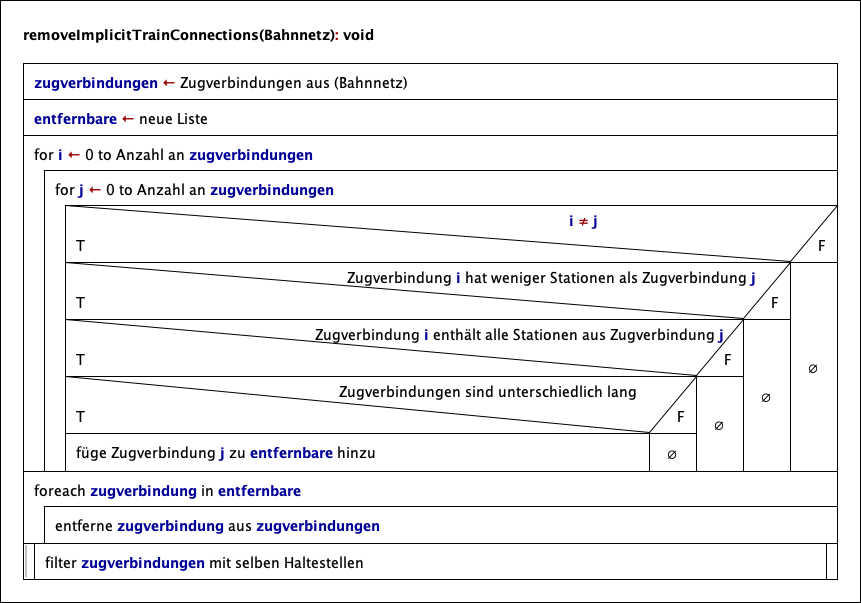
\includegraphics[width=\linewidth]{images/Struktogramme/reducer/reduction3/removeImplicitTrainConnections.png}
    \captionof{figure}{Entfernen von impliziten Zugverbindungen}
    \label{pro:subsubsecpar:entfernen-von-impliziten-zugverbindungen}
\end{center}

\begin{center}
    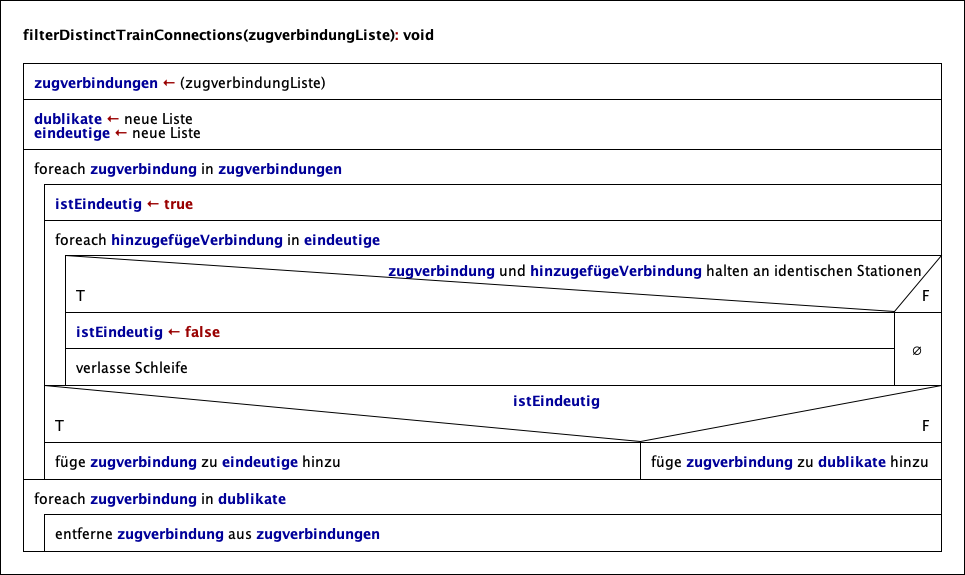
\includegraphics[width=\linewidth]{images/Struktogramme/reducer/reduction3/filterDistinctTrainConnections.png}
    \captionof{figure}{Entfernen von identischen Zugverbindungen}
    \label{pro:subsubsecpar:ueberpruefung-ob-zugverbindung-implizit-ist}
\end{center}

\newpage
\subsubsection{Algorithmus}\label{pro:subsubsec:algorithmus}
\begin{center}
    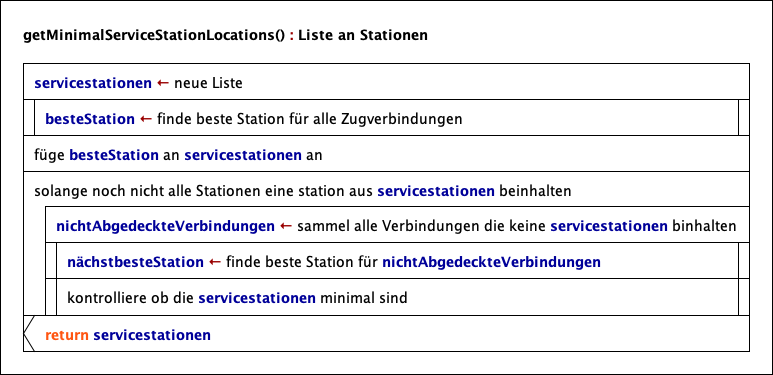
\includegraphics[width=\linewidth]{images/Struktogramme/algorithm/getMinimalServiceStationLocations.png}
    \captionof{figure}{Berechne minimale Anzahl an Servicestationen}
    \label{pro:subsubsecpar:berechne-minimale-anzahl-an-servicestationen}
\end{center}

\begin{center}
    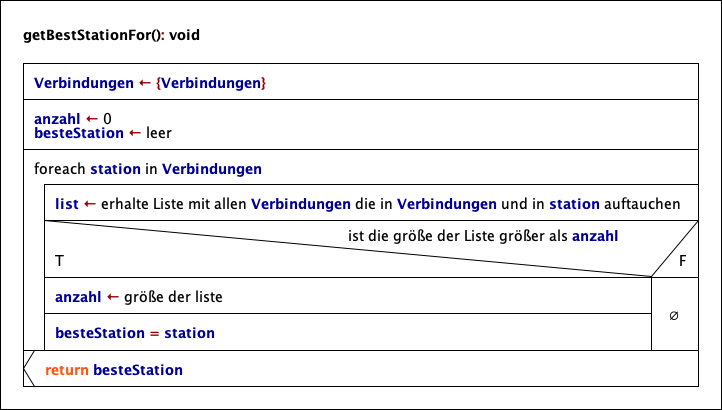
\includegraphics[width=\linewidth]{images/Struktogramme/algorithm/getBestStationFor.png}
    \captionof{figure}{Berechne beste Station für übergebene Zugverbindungen}
    \label{pro:subsubsecpar:berechne-minimale-anzahl-an-servicestationen}
\end{center}

\begin{center}
    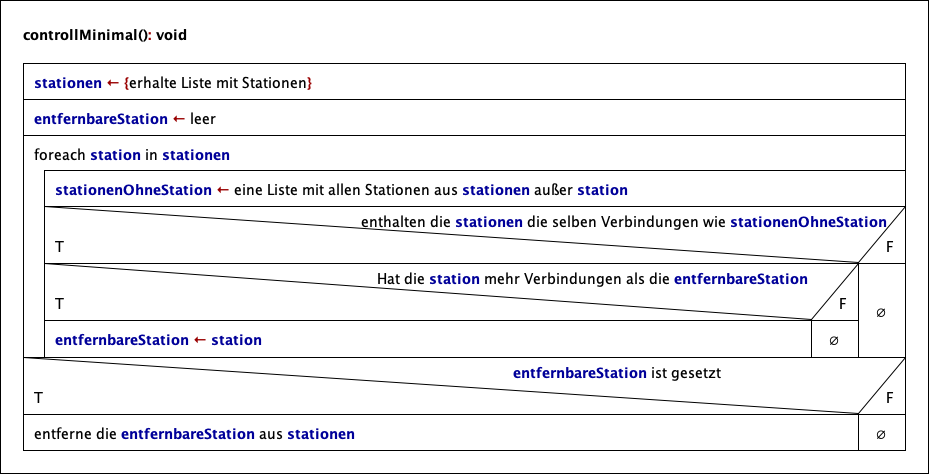
\includegraphics[width=\linewidth]{images/Struktogramme/algorithm/controllMinimal.png}
    \captionof{figure}{Überprüfe minimale Anzahl an Servicestationen}
    \label{pro:subsubsecpar:ueberpruefe-minimale-anzahl-an-servicestationen}
\end{center}

\section{Entwicklungsdokumentation}\label{pro:sec:entwicklerdokumentation}
Die Dokumentation des Programms wurde in Javadoc vorgenommen und kann im Ordner javadoc eingesehen werden.
Hierzu kann die index.html aufgerufen werden
%    \addtocontents{toc}{\protect\newpage}
    \chapter{Testdokumentation}\label{ch:testdokumentation}

\section{Systemtests}\label{test:sec:systemtests}
Die Systemtests wurden mit Hilfe der Testdateien durchgeführt.\\
Im Folgenden wird auf die Systemtest mit den Testdateien eingegangen. Dazu wurden sich entsprechende Äquivalenzklassen überlegt und jeweils mit einem Vertreter dieser Klassen eine Testdatei erstellt und ein Test durchführt.\\
\subsection{Normalfälle}\label{test:sec:normalfaelle}
\begin{center}
    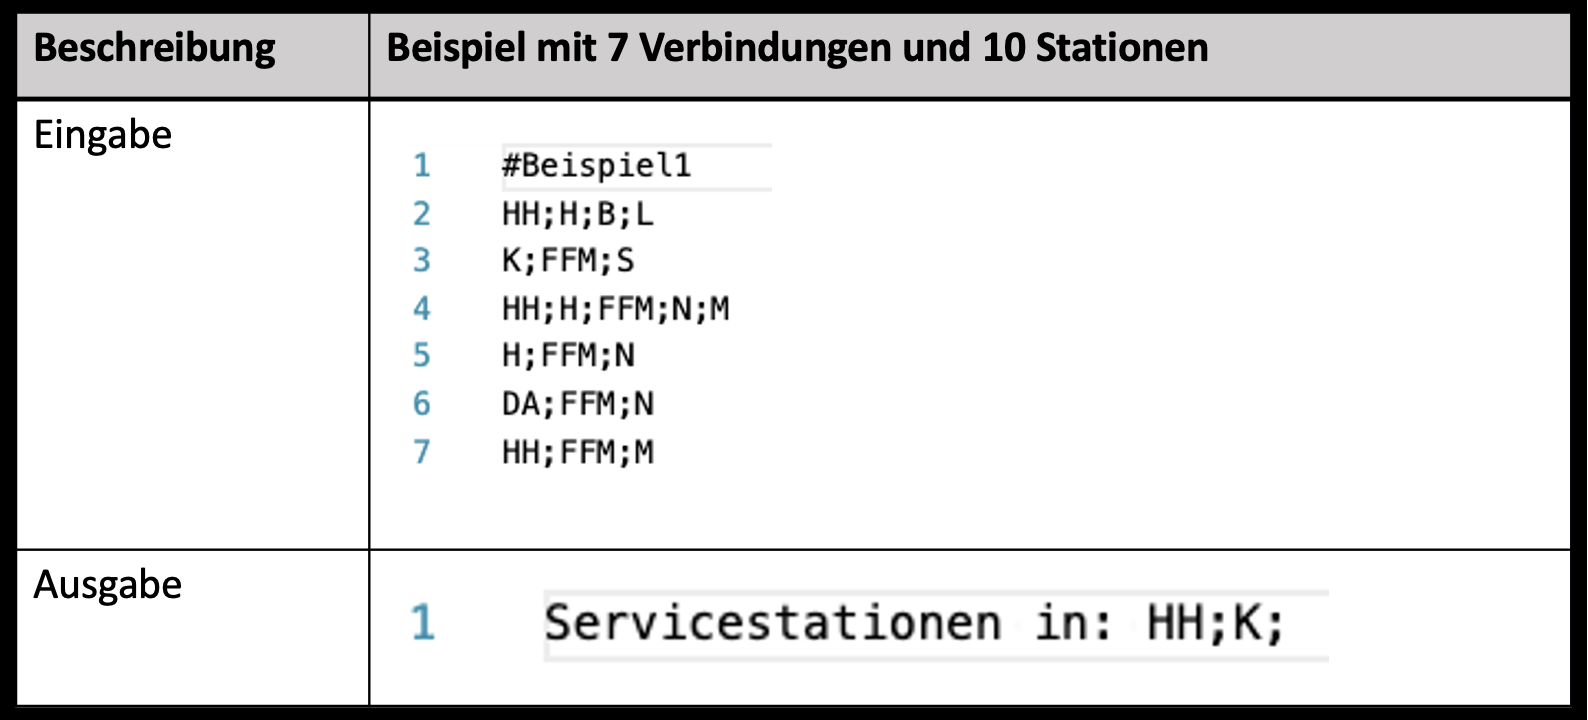
\includegraphics[width=\linewidth]{images/Tests/IHK-Beispiele/Beispiel1.png}
    \label{test:subsecpar:beispiel1}
\end{center}

\begin{center}
    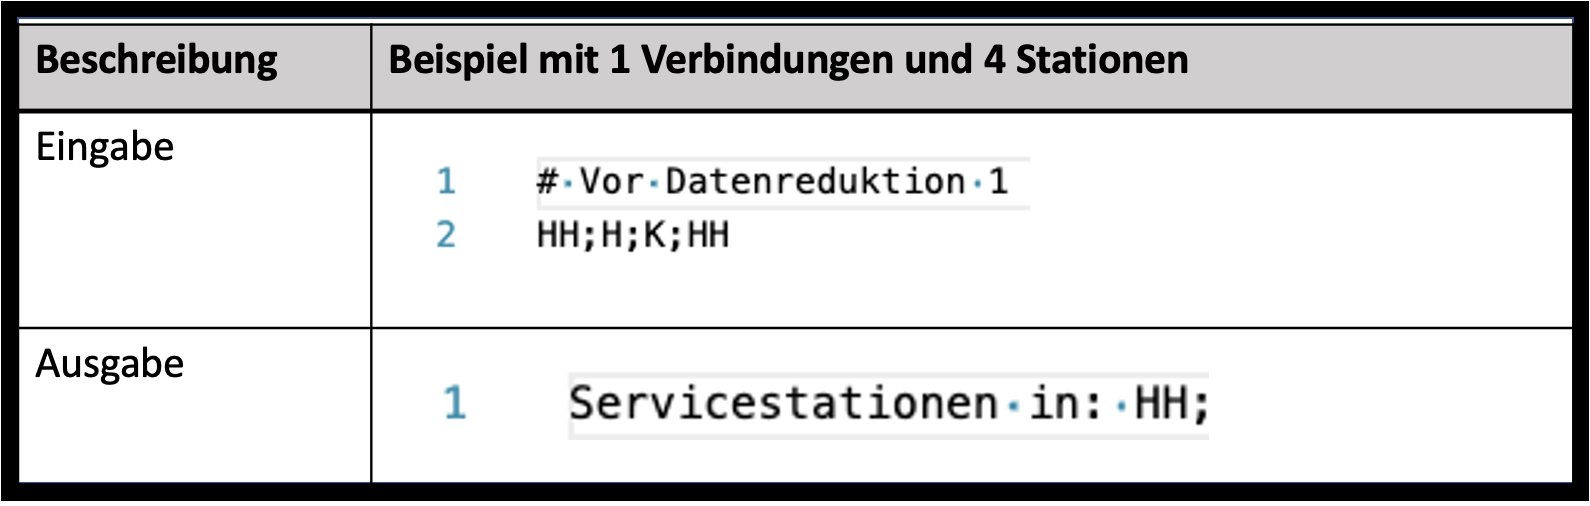
\includegraphics[width=\linewidth]{images/Tests/IHK-Beispiele/Datenreduktion1.png}
    \label{test:subsecpar:Datenreduktion1}
\end{center}

\begin{center}
    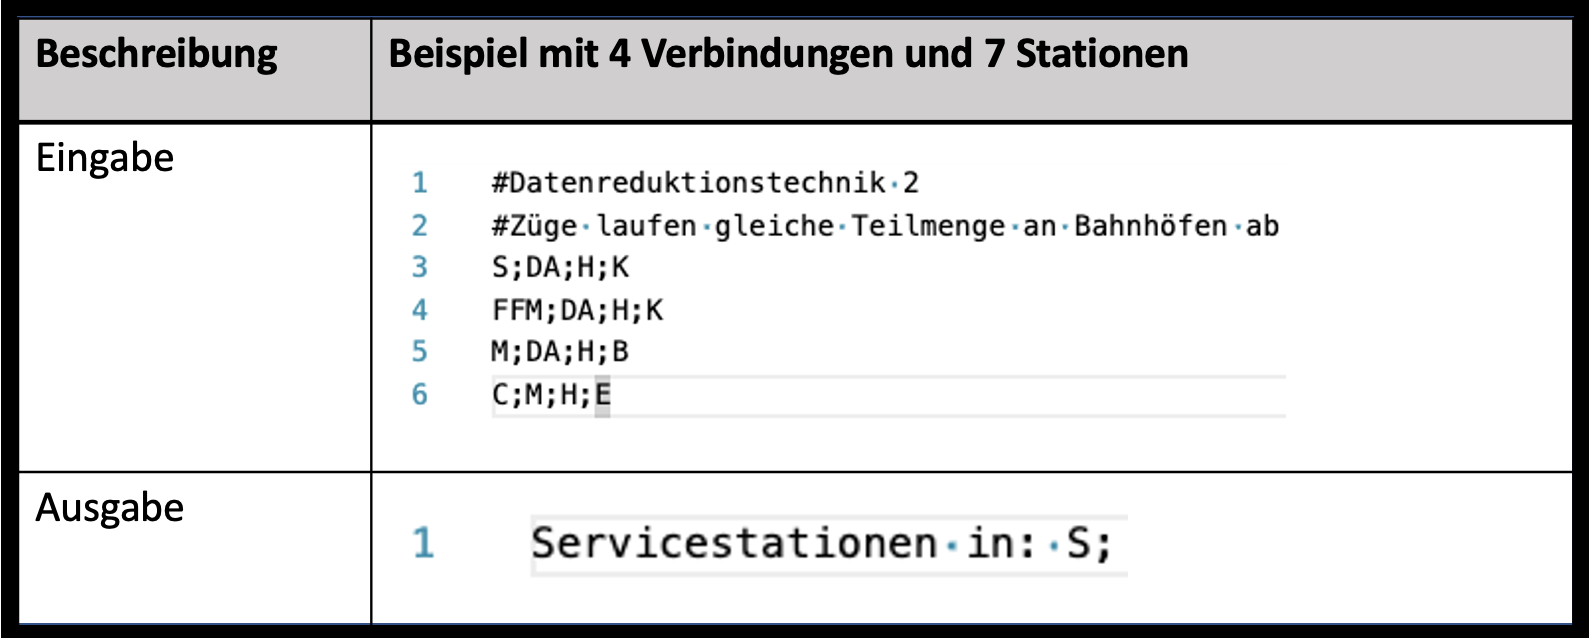
\includegraphics[width=\linewidth]{images/Tests/IHK-Beispiele/Datenreduktion2.png}
    \label{test:subsecpar:Datenreduktion2}
\end{center}

\begin{center}
    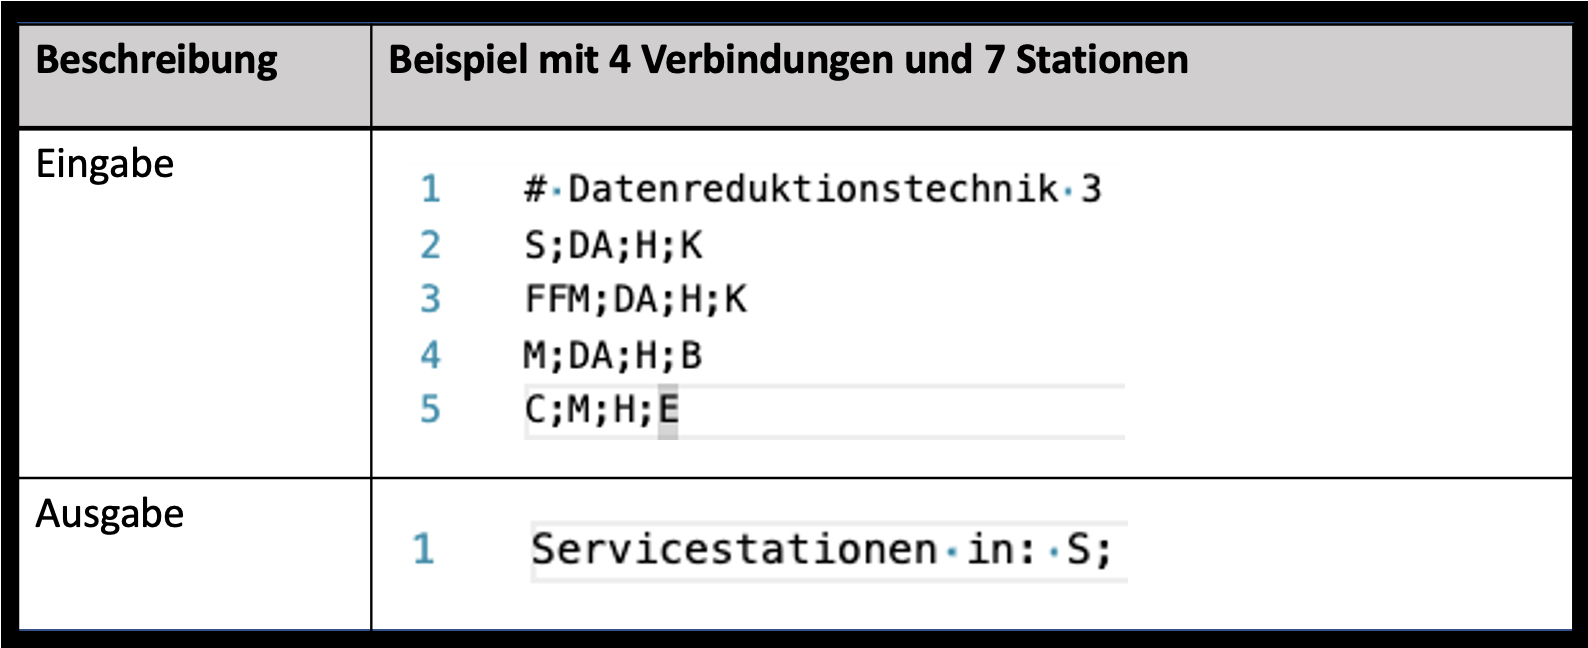
\includegraphics[width=\linewidth]{images/Tests/IHK-Beispiele/Datenreduktion3.png}
    \label{test:subsecpar:Datenreduktion3}
\end{center}


\subsection{Fehlerfälle}\label{test:sec:fehlerfaelle}
Die folgenden Test decken die in \ref{auf:sec:fehlerarten} gennanten Fehlerfälle ab.

\subsubsection{Technische Fehler}\label{test:sec:technische-fehler}
\begin{center}
    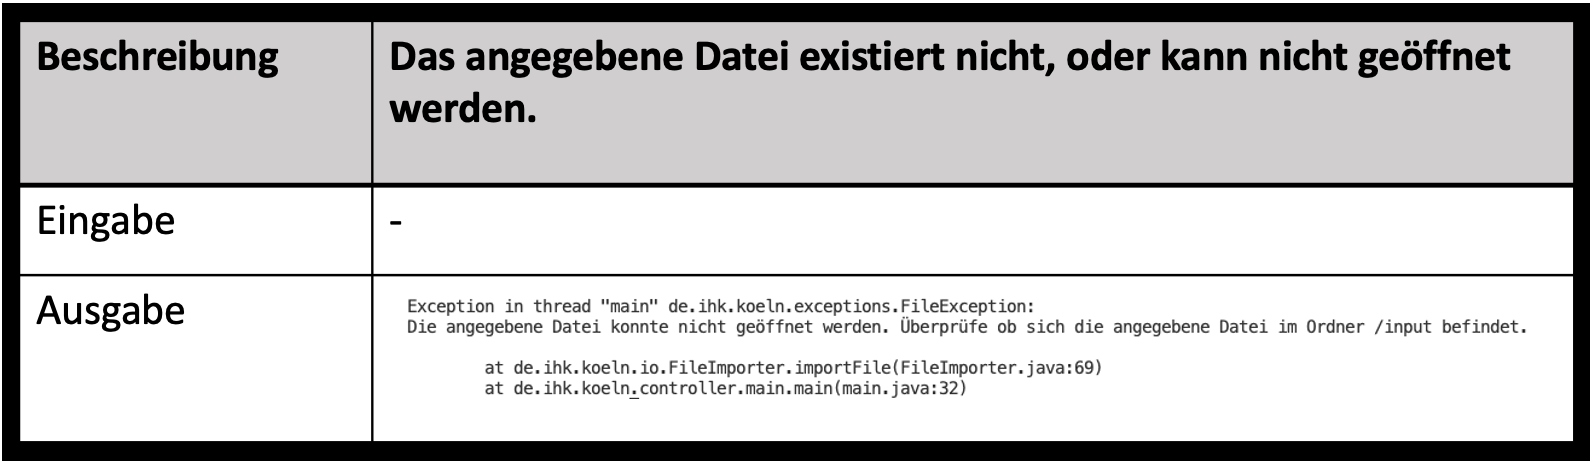
\includegraphics[width=\linewidth]{images/Tests/Fehlerfälle/FileException.png}
    \label{test:subsecpar:einlese-fehler}
\end{center}

\begin{center}
    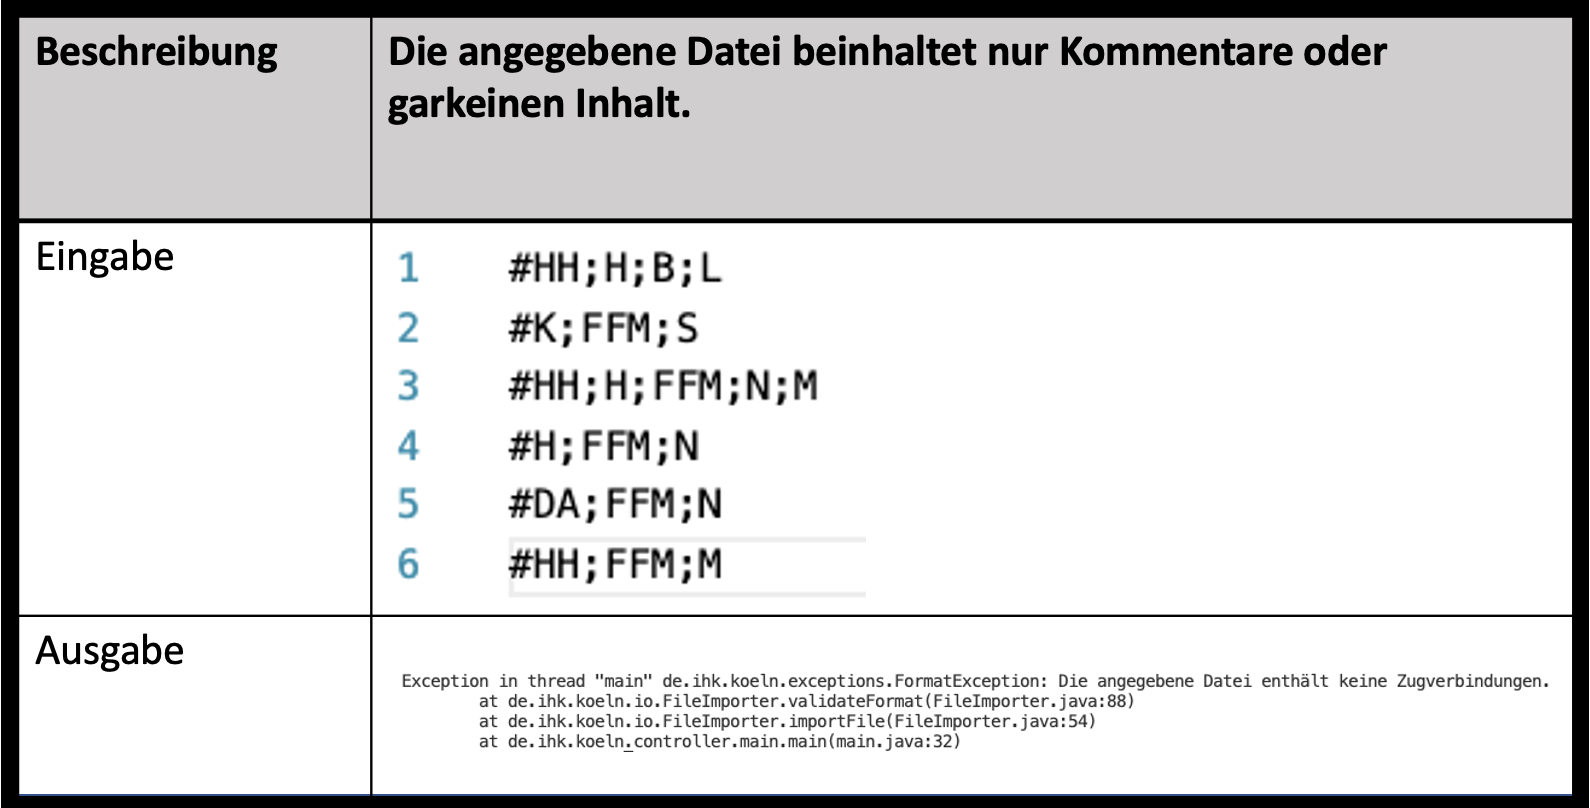
\includegraphics[width=\linewidth]{images/Tests/Fehlerfälle/LerreDatei.png}
    \label{test:subsecpar:leere-datei}
\end{center}

\subsubsection{Syntaktische Fehler}\label{test:sec:syntaktische-fehler}
\begin{center}
    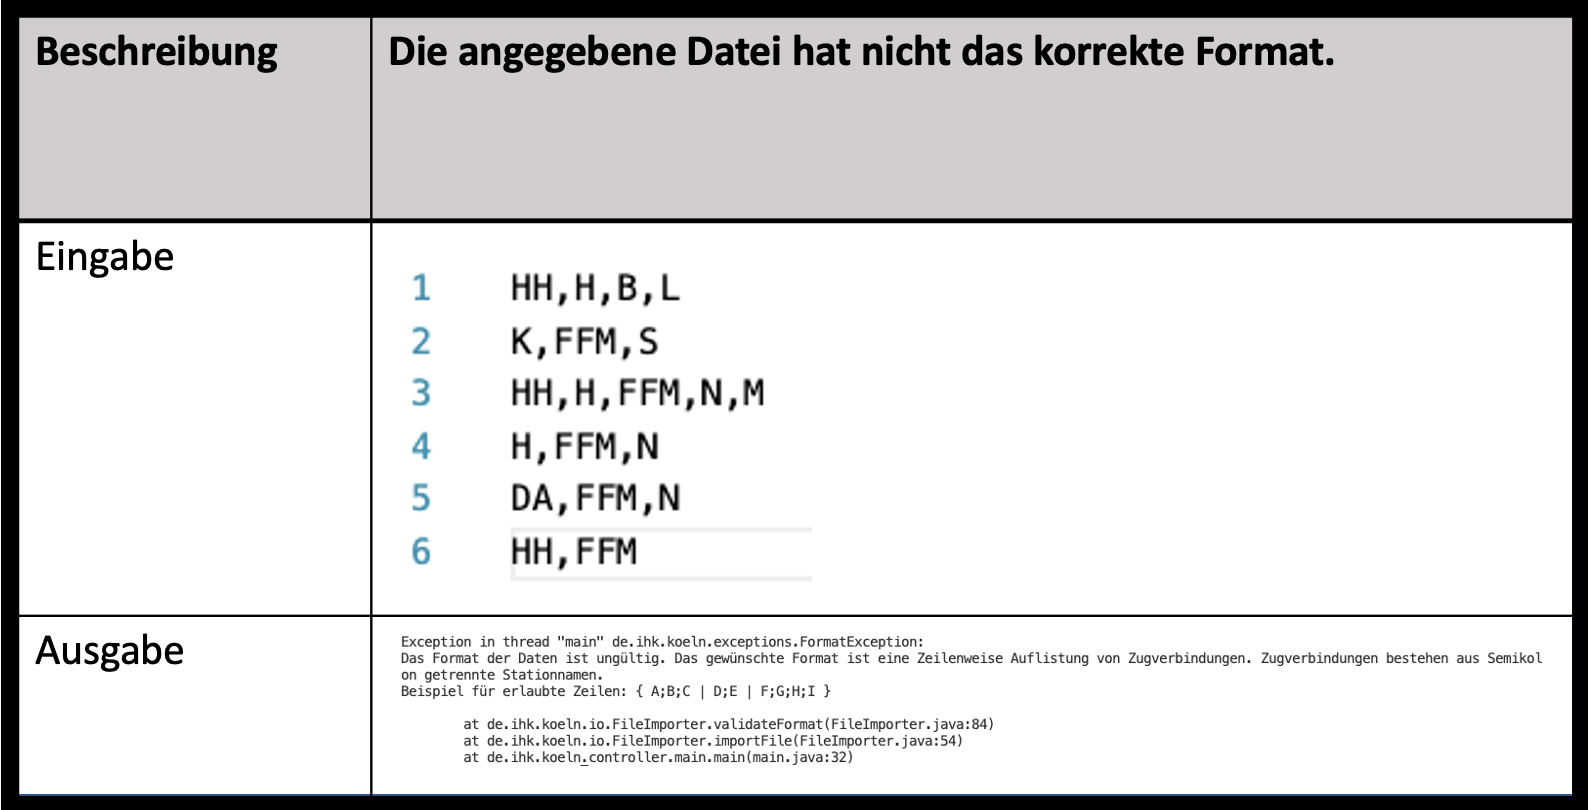
\includegraphics[width=\linewidth]{images/Tests/Fehlerfälle/FormatException.png}
    \label{test:subsecpar:format-fehler}
\end{center}

\subsubsection{Semantische Fehler}\label{test:sec:semantische-fehler}
\begin{center}
    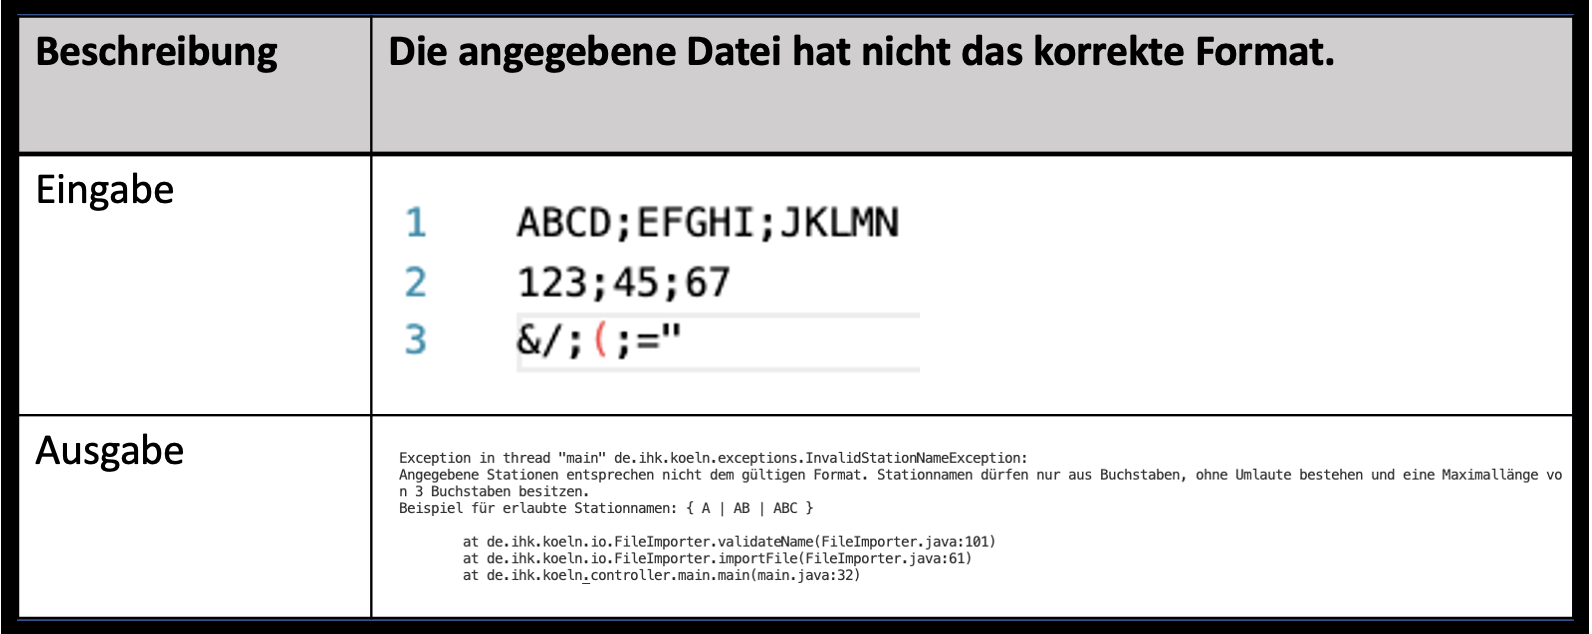
\includegraphics[width=\linewidth]{images/Tests/Fehlerfälle/InvalidNameException.png}
    \label{test:subsecpar:namen-sind-nicht-erlaubt}
\end{center}

\subsection{Grenzfälle}\label{test:sec:grenzfaelle}

\begin{center}
    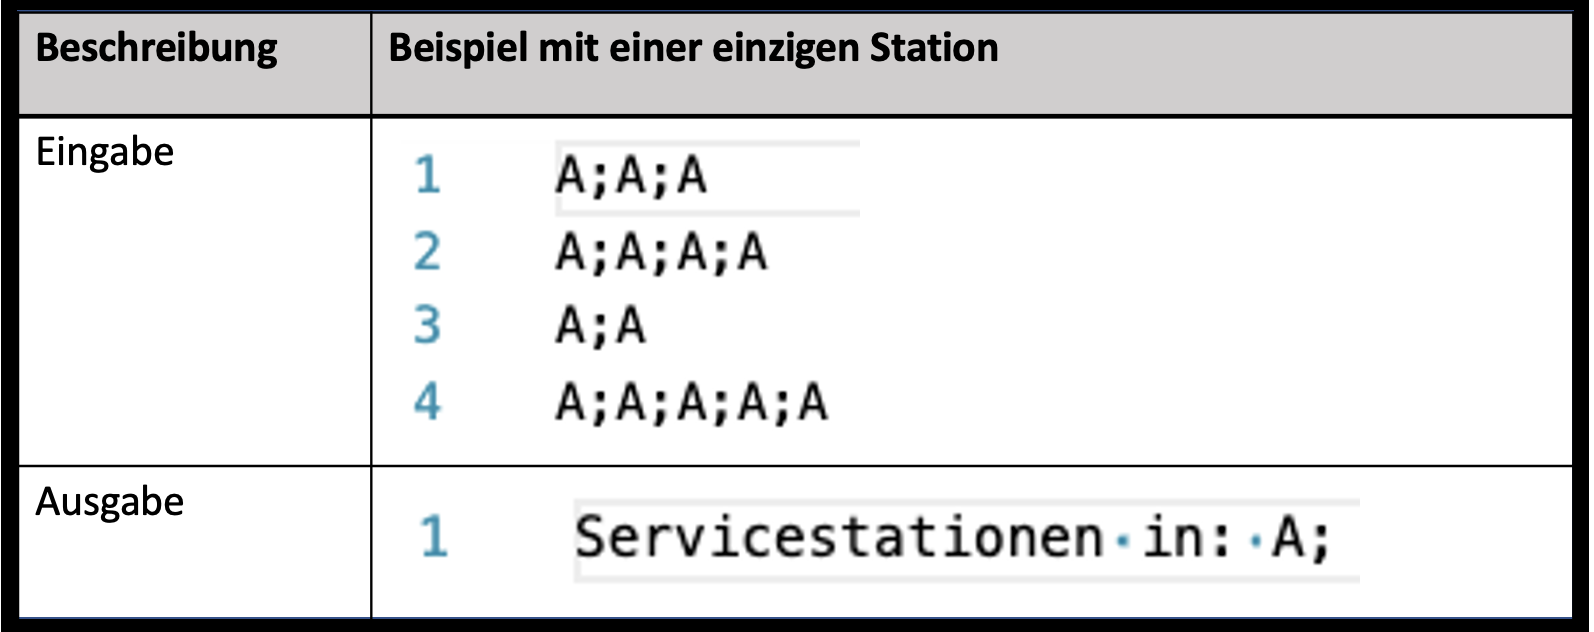
\includegraphics[width=\linewidth]{images/Tests/Grenzfälle/einzigeStation.png}
    \label{test:subsecpar:einzige-station}
\end{center}

\begin{center}
    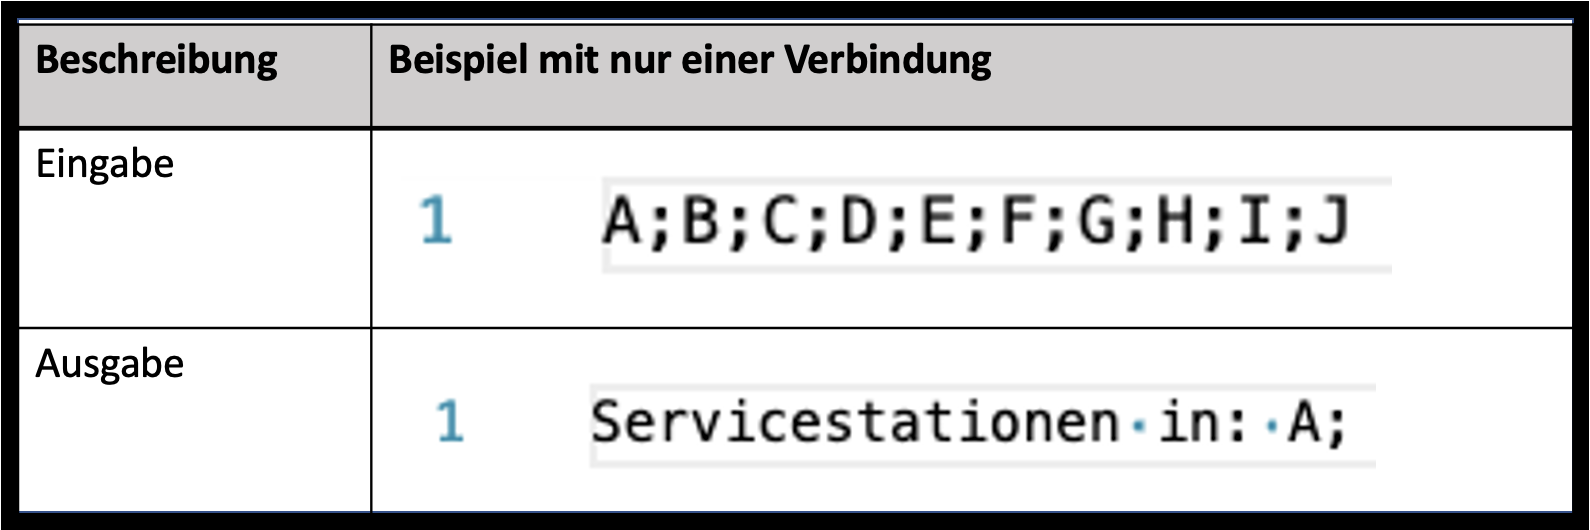
\includegraphics[width=\linewidth]{images/Tests/Grenzfälle/einzigeVerbindung.png}
    \label{test:subsecpar:einzige}
\end{center}


\subsection{Sonderfälle}\label{test:sec:sonderfaelle}

\begin{center}
    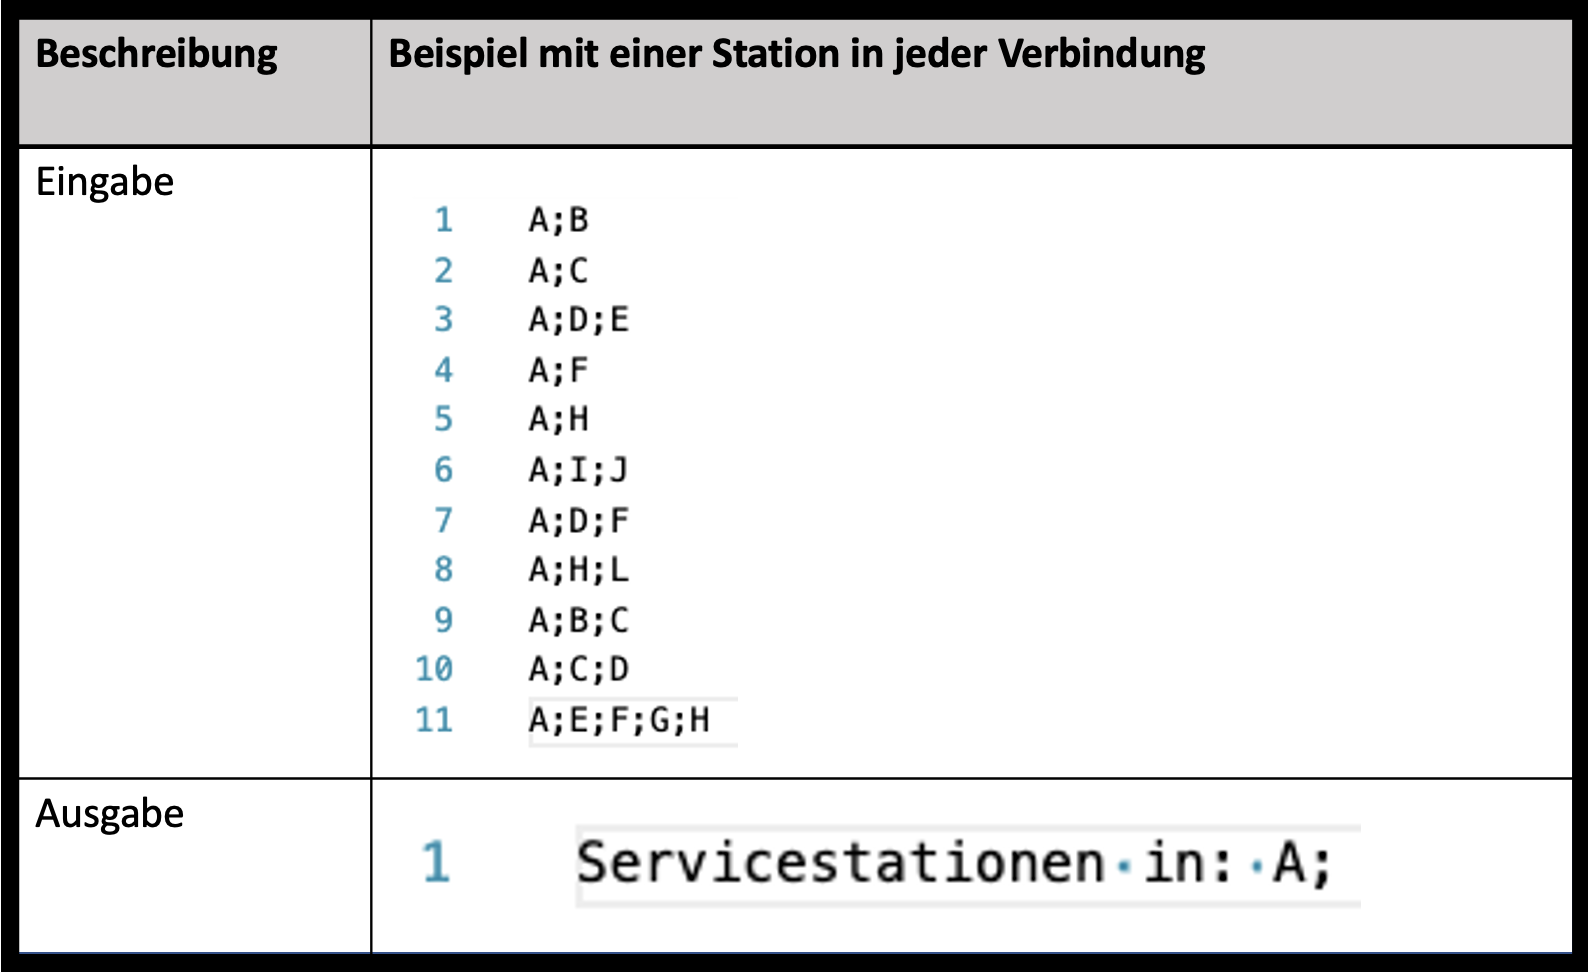
\includegraphics[width=\linewidth]{images/Tests/Sonderfälle/uerbergreifendeStation.png}
    \label{test:subsecpar:uerbergreifendeStation}
\end{center}

\begin{center}
    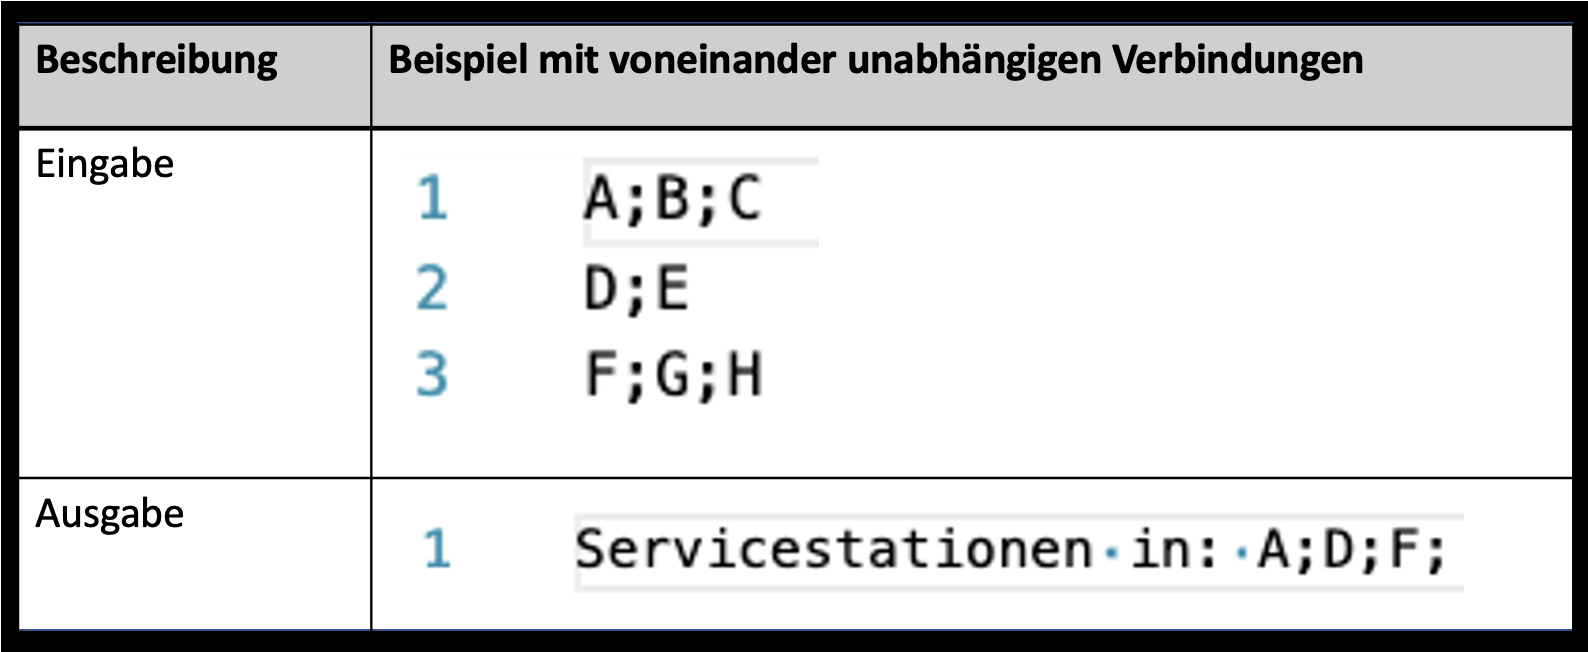
\includegraphics[width=\linewidth]{images/Tests/Sonderfälle/unabhaengigeStationen.png}
    \label{test:subsecpar:unabhaengigeStationen}
\end{center}


\section{Ausführliches Beispiel}\label{test:sec:ausfuehrliches-beispiel}
Im folgendem wird für ein Bahnnetz ein kompletter Algorithmen durchlauf beschrieben.\\

Dafür wird folgende Datei eingelesen:\\
\begin{center}
    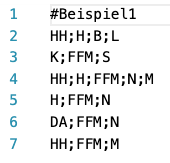
\includegraphics[width=\linewidth]{images/Programmdurchlauf/eingabedatei.png}
    \label{test:subsecpar:eingabedatei}
\end{center}

Beim lesen der Datei werden Kommentare ignoriert und die Zeilen in Zugverbindungen umgewandelt. Dabei wird auf korrekte Syntax geachtet.
Sind alle Verbindungen eingelesen werden die Stationen ermittel. Zusammen werden diese in einem Zugnetz gespeichert. Das vorliegende Zugnetz liegt folgendermaßen vor:\\

\begin{center}
    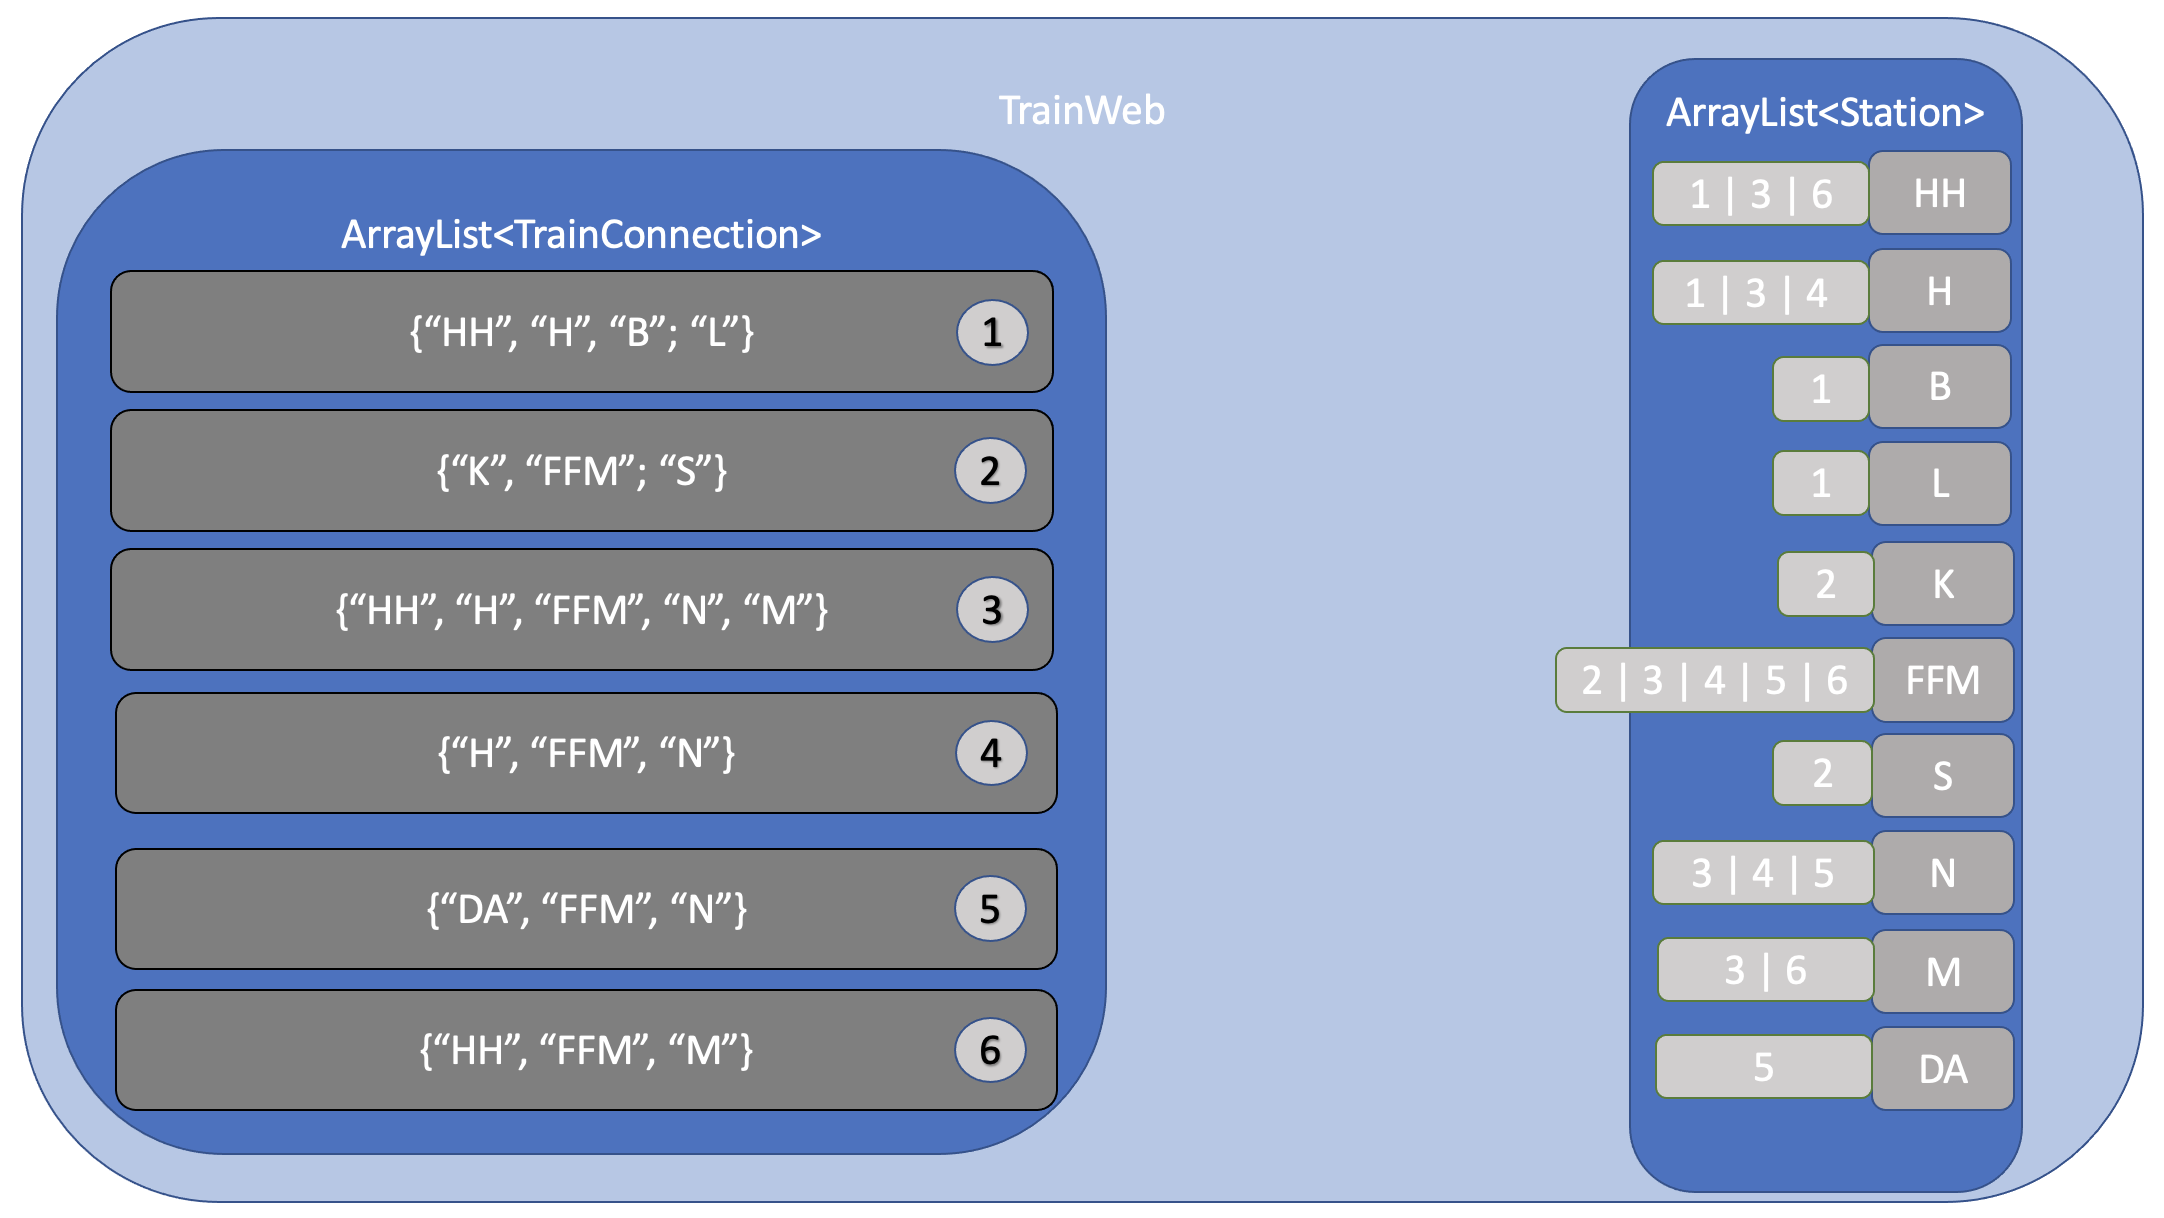
\includegraphics[width=\linewidth]{images/Programmdurchlauf/Datenstruktur01.png}
    \label{test:subsecpar:datenstruktur1}
\end{center}
\\
Diese Zugnetz wird nun Reduziert. Dafür werden die drei Reduktionsverfahren angewandt.\\
Die erste Reduktiontechnik überprüft ob eine Station mehrfach in einer Zugverbindung vorkommt. Ist dies der Fall werden alle doppelten vorkommen entfernt.\\
Da in diesem Fall keine doppelten Stationen vorkommen, wird das Netz nicht verändert.\\
\\
Die zweite Reduktionstechnik fasst Stationen zusammen, die keinen Aussagewert h aben. Dies ist dann der Fall, wenn jede Verbindung die Station A anfährt auch eine Station B beinhaltet. In diesem Fall kann Station A gelöscht werden.\\
Stationen \texttt{K}, \texttt{S}, \texttt{B}, \texttt{L} und \texttt{DA} tauchen in jeweils nur einer Verbindung vor. Solang diese noch weiter Stationen beinhalten können diese sofort entfernt werden. Betrachtet man Station \texttt{M} und \texttt{N} lässt sich feststellen, dass diese in allen Verbindungen auch \texttt{FFM} anfahren und somit ebenfalls entfernt werden können.\\
Das Bahnnetz liegt nun folgendermaßen vor:\\

\begin{center}
    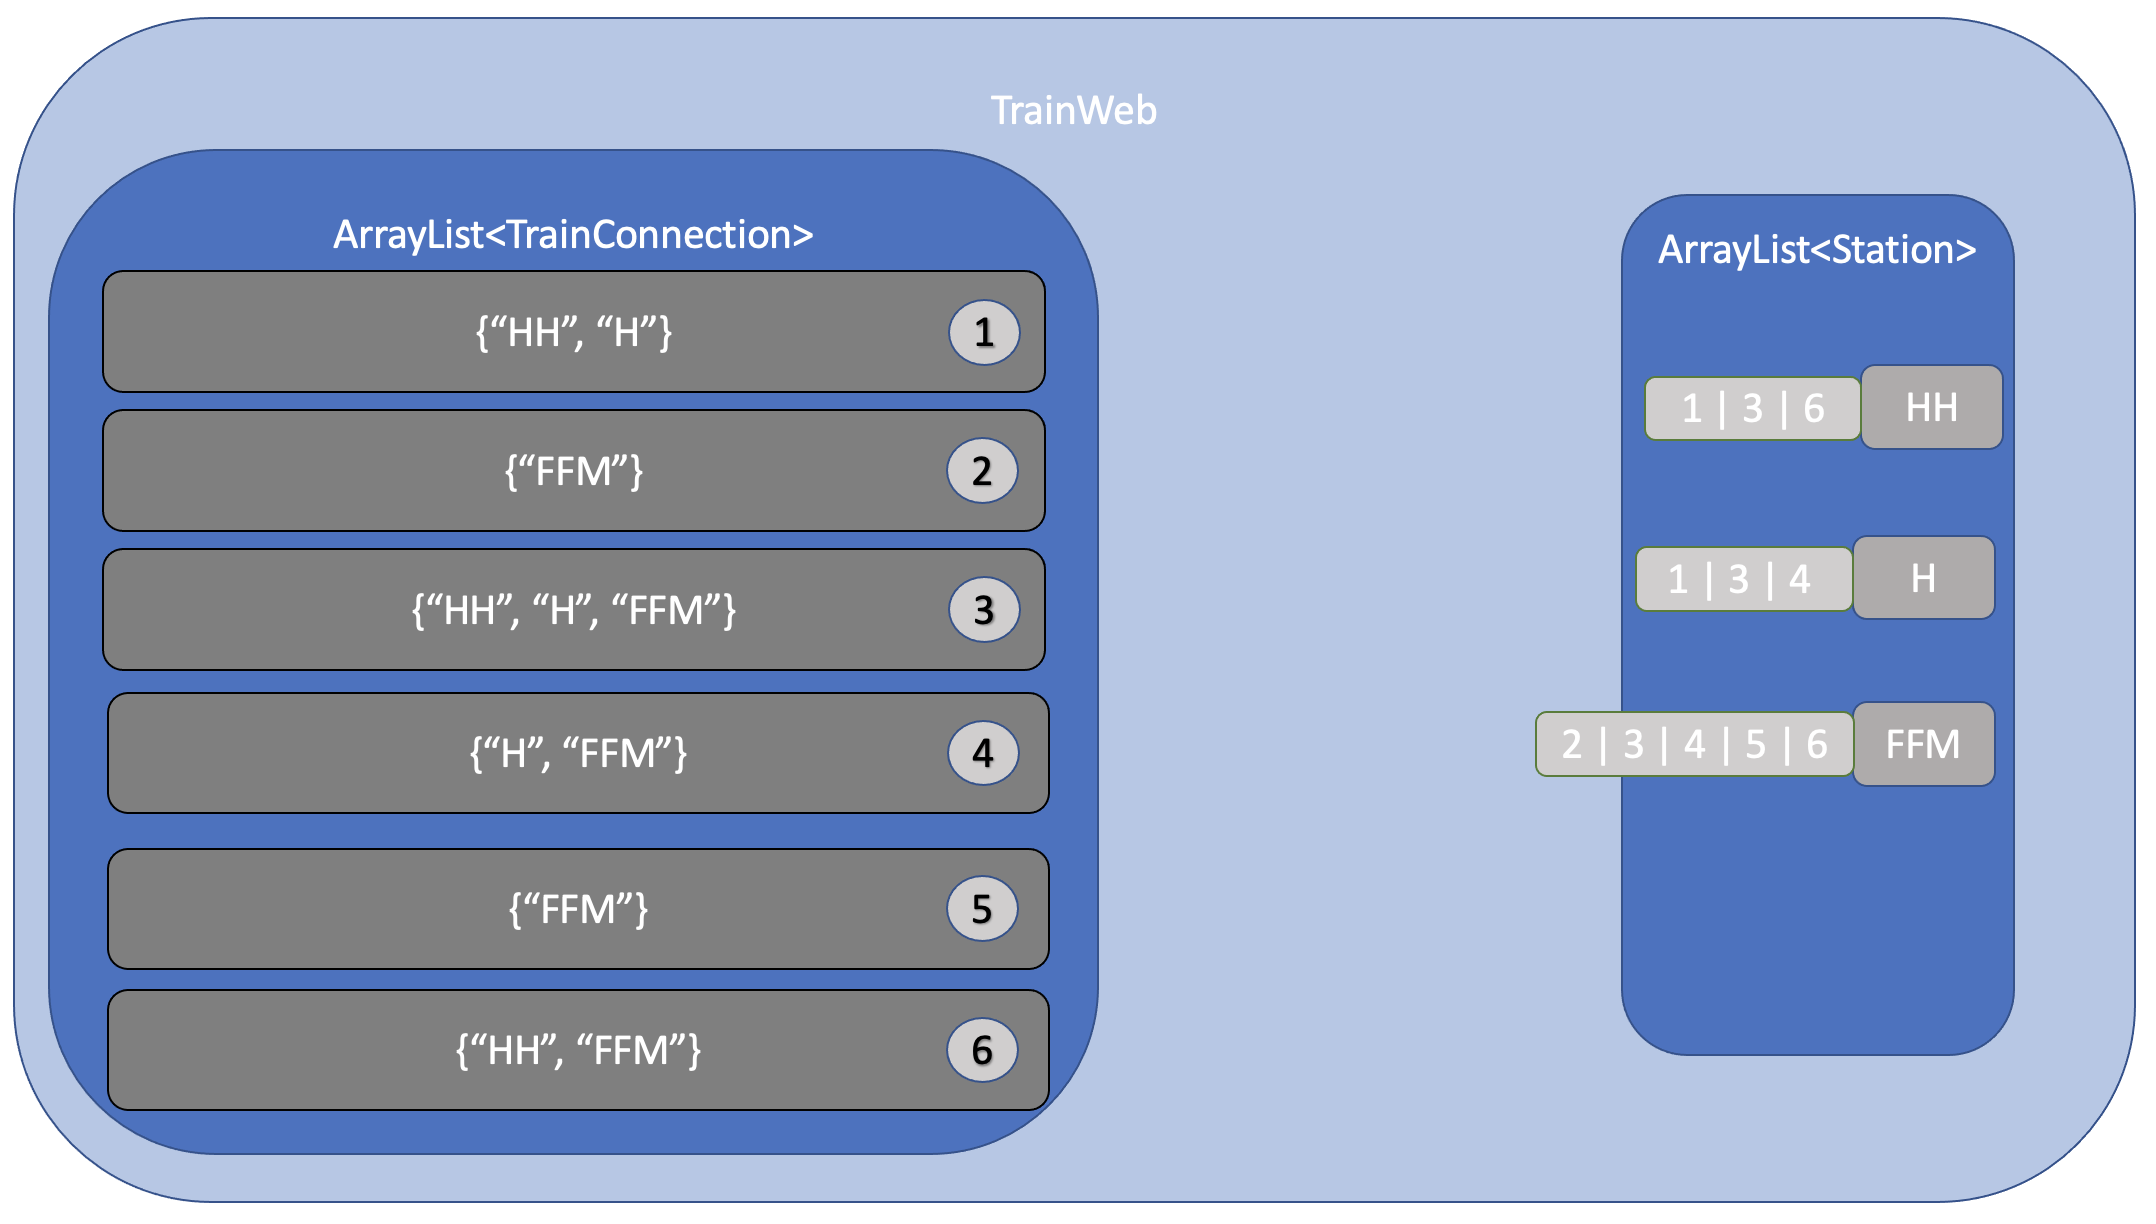
\includegraphics[width=\linewidth]{images/Programmdurchlauf/Datenstruktur02.png}
    \label{test:subsecpar:datenstruktur2}
\end{center}

Die dritte Reduktionstechnik überprüft ob eine Zugverbindung implizit in einer anderen Zugverbindung enthalten ist. Ist dies der Fall kann die größere Zugverbindung entfernt werden. Das gilt auch für Verbindungen die die genau selben Stationen anfahren.\\
In diesem Fall können alle Verbindungen die die Station \texttt{FFM} anfahren entfernt werden, da Verbindung 2 und 5 nur \texttt{FFM} beinhalten. Dabei muss ebenfalls nur eine der beiden Verbindungen gespeichert werden.\\
Die übergebliebenen Verbindungen ergeben folgendes Bahnnetz:\\

\begin{center}
    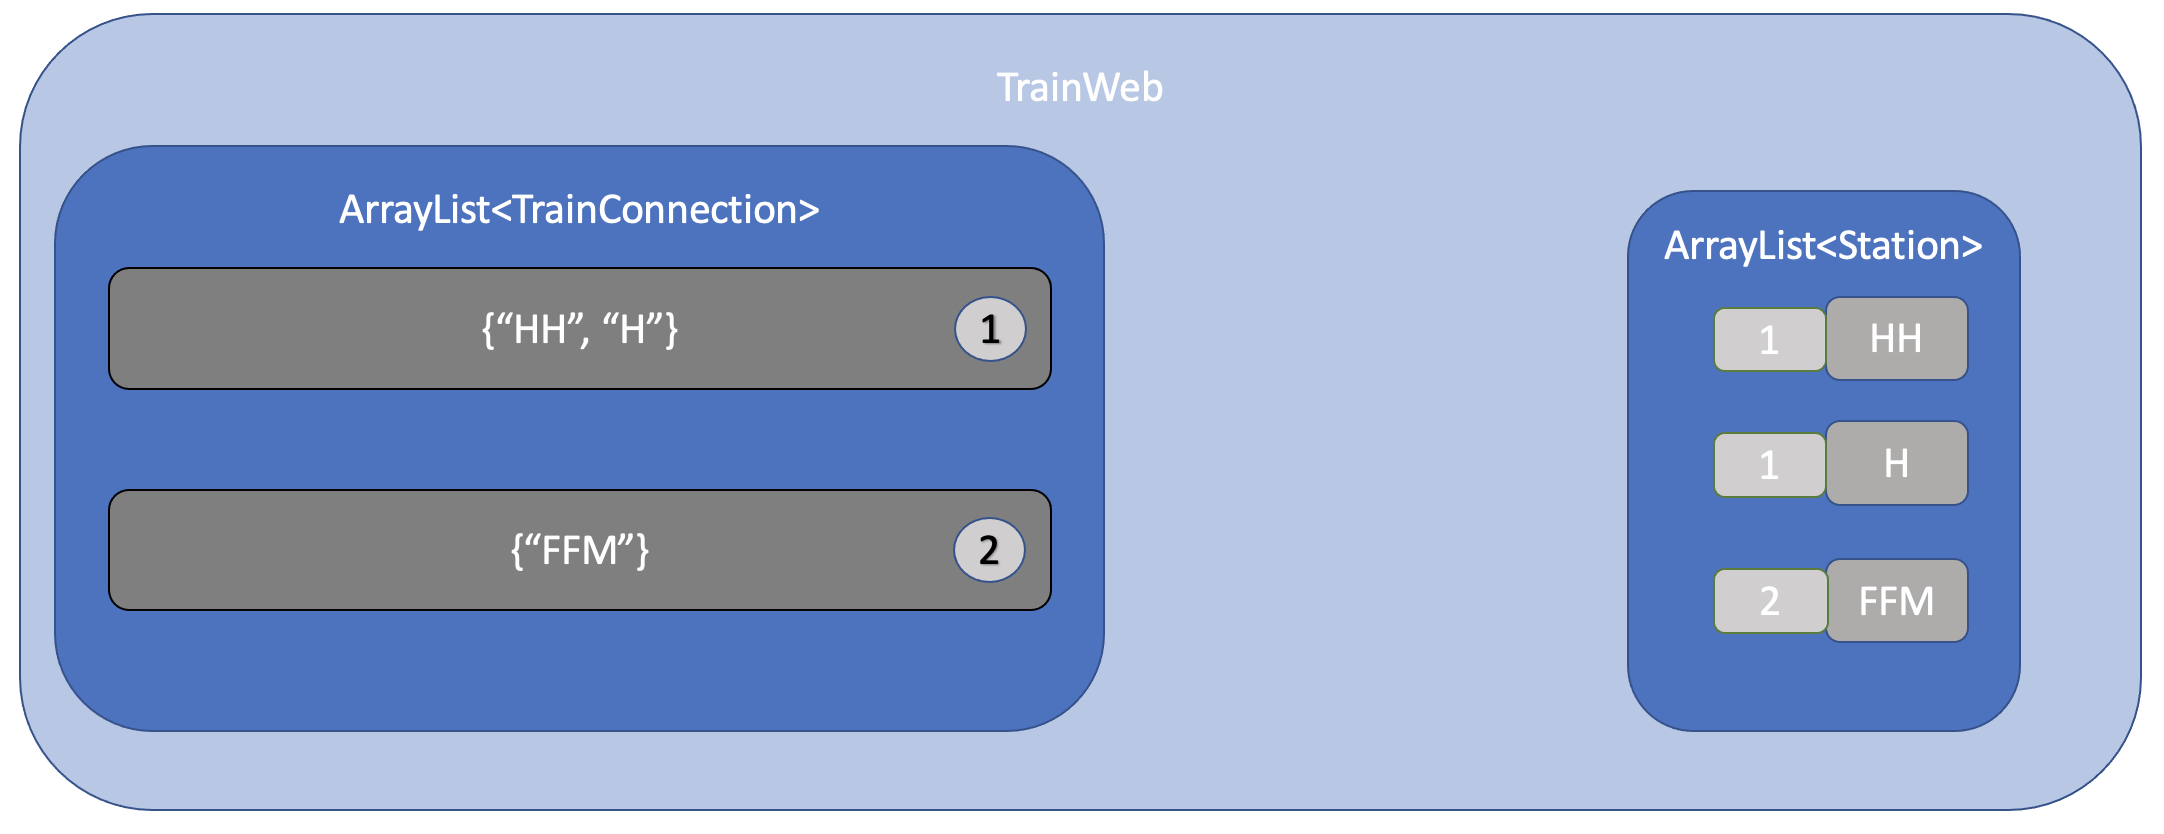
\includegraphics[width=\linewidth]{images/Programmdurchlauf/Datenstruktur03.png}
    \label{test:subsecpar:datenstruktur2}
\end{center}
\\
Das nun reduzierte Bahnnetz kann jetzt dem Algorithmus übergeben werden, welcher die Stationen ausgewählt, die als Servicestation verwerndet werden können.\\
Dafür wir die Station ausgewählt, die in den meisten Verbindungen vorkommt. In diesem Fall haben alle Stationen gleich viele Verbindungen sodass eine beliebige Station gewählt werden kann. Wir\\
    \chapter{Zusammenfassung und Ausblick}\label{ch:zusammenfassung-und-ausblick}


\section{Zusammenfassung}\label{sec:zusammenfassung}
Es wurde ein Programm entwickelt, welches die Berechnung von Servicestationen wie gefordert umsetzt.
Eingabe, Verarbeitung und Ausgabe laufen in voneinander unabhängigen Prozessen. Beliebige Datensätze können dem Programm übergeben. Die Verarbeitung erfolgt in zwei Schritten in dem zunächst eine optionale Reduktion auf die Eingabedaten durchgeführt wird und anschließend die eigentliche Berechnung stattfindet. Das Programm endet, wenn das gefundene Ergebnis ausgegeben wurde.\\
Die angesprochenen Teilaufgaben wurden in einzelne Klassen aufgeteilt. Diese können unabhängig voneinander verändert und erweitert werden.
Die Verfahren und ihre Details wurden ausführlich dokumentiert. Die Wahl von unterschiedlichen Datenstrukturen wurde begründet und der Programmentwurf ist durch diverse UML- und Nassi-Shneiderman-Diagramme gut nachvollziehbar. Für Entwickler wurde eine Dokumentation direkt im Source-Code erstellt.

\section{Ausblick}\label{sec:ausblick}
\subsection{Einführung von Pattern}\label{sec:pattern}
Wie bereits angesprochenen sind alle Teilaufgaben systematisch getrennt. Hier bietet es sich an ein Stategie-Pattern zu implementieren. Dieses würde es ermöglichen die einzelnen Teilaufgaben austauschbar zu machen. Außerdem ist ein Rahmen gegeben sodass Veränderungen keinen Einfluss auf die Benutzung der einzelnen Komponenten haben können.\\

\subsection{Algorithmus}\label{sec:algorithmus}
Der implementierte Algorithmus glänz mit Laufzeiteffizienz. Er ist in der Lage ein Bahnnetz mit 10.000 Verbindungen und 500 Staitionen in bis zu 5:11:29 Minuten auszurechnen. Je nach Hardware kann dies varieren.\\
Beim Vergleich mit anderen Algorithmen ist jedoch aufgefallen, dass nicht immer die minimale Anzahl an Servicestationen ermittelt wird. Dies stellt logischerweise ein Problem dar und sollte dringend ausgebessert werden.\\

Dafür bieten sich folgende Ansätze an. \\

\subsubsection{Reiner Brute-Force Ansatz}\label{sec:brute-force}
Um sicher zu gehen, immer ein minimales Ergebnis zu erhalten, kann ein Brute-Force Ansatz implementiert werden. Dieser würde alle möglichen Kombinationen an Lösungsstationen durchgehen und die Lösung mit der geringsten Anzahl an Stationen ausgeben. Auf unkomplexe Bahnnetze können bei diesem Ansatz gute Ergebnisse erzielt werden. Da es sich beim Brute-Force Ansatz jedoch um ein expondenzielles Verfahren handelt, ist die Laufzeit bei komplexeren Bahnnetzen nicht wünschenswert.\\
Dies gilt auch wenn ein Abbruchkriterium eingebaut wird, welches neue Ergebnisse durch das aktuell beste Ergebnis einschränkt. Damit werden nurnoch Kombinationen überprüft, die eine Verbesserung zum aktuellen Ergebnis ermöglichen können. Auch hier müssen jedoch Laufzeiteinbussen in kauf genommen werden\\

\subsubsection{Erweiterung durch Brute-Force}
Um von der Laufzeiteffizienz des aktuellen Algorithmus zu profitieren und trotzdem ein tatsächlich minimales Ergebnis zu erhalten, kann der Algorithmus um einen Brute-Force Ansatz erweitert werden. Dafür wird das Ergebnis der des Greedy-Algorithmus mit einem Brute-Force Ansatz validiert.\\
Dazu werden wird die Liste an Servicestationen überprüft und für jede möglichen Stations Kombination ermittelt. Diese werden dann ebenfalls mit allen Kombinationen von allen verfügbaren Stationen verglichen. Bedingung ist das die Auswahl an Bahnstation kleiner ist als die der aktuellen Service Stationen. Sollten beide Kombinationen die selben Verbindungen abdecken, wird die neue Kombination als mit den betrachteten Servicestationen getauscht.\\
Sollten keine Tauschmöglichkeiten mehr gefunden werden ist davon auszugehen eine tatsächlich minimal Anzahl an Staionen gefunden zu haben.\\
Auch dieser Ansatz ist expondenziell. Durch eine bereits approximierte Lösung ist jedoch davon auszugehen, dass weniger Vergleiche getätigt werden müssen und die Laufzeit besser wird.\\

\subsection{Testabdeckung}\label{sec:testabdeckung}
Die hier dokumentierten Test, testen nur einen erfolgreichen oder auch fehlerhaften Durchlauf des Programms. Da die Projektstruktur eine saubere Trennung der einzelnen Komponenten gewährleistet, bietet es sich an diese mit Unit-Tests zu testen.\\
    % ============= Buchstabenteil ==============
    \renewcommand{\thechapter}{\Alph{chapter}}%
    \setcounter{chapter}{0}
    \chapter{Abweichung und Ergänzung}\label{ch:abweichung-und-ergaenzung}

\section{Probleme}
Im Verlaufe der Implemeniterung ist aufgefallen, dass manche Projektabschnitte in der Klausur falsch verstanden wurden. In der folge dessen wurden falsche schlüße gezogen.\\

\subsection{Datenreduktionsverfahren 2}
Ein Beispiel ist die zweite Reduktionsmethode. Diese entfernt nicht nur, wie zunächst angenommen, benachtbarte Stationen. Die Reihenfolge der Stationen ist bei der Reduktion hinfällig. Dadurch gibt es massive unterschiede in der implementierung der zweiten Redukitonsmethode.\\

\subsection{Algorithmus}
Innerhalb der Klausur sind gedanklich die Stationen und Verbindungen miteinander verschmolzen. Teilweise werden Verfahren dadurch falsch gefolgert und falsch dargestellt.


\section{Datenstrukturen}
Um ein Übersichtliches System zu schaffen, wurden in der Strukturierung auf mögliche Hilfsklassen verzichtet. Damit sollte die leserlichkeit erhalten bleiben und die Struktur Übersichtlich gestalten.\\
Dieser Ansatz wurde aus mehreren Gründen verworfen.\\
\subsection{Trennung von Speicher und Verarbeitung}
Die geplante Modell Klasse sollte ursprünglich nicht nur die Daten speichern sondern ebenfalls die Reduktionsverfahren wie auch den Algorithmus berechnen. Dies führte zu Übersichts Problemen. Erster Ansatz war nun das Datenmodell und die Verfahren zu trennen.\\ 

\subsection{Trennung der Verfahren}
Dadurch konnten Klassen deutlich reduziert werden. Die gewünschte Übersicht war immernoch nicht gegeben. Dies führte zur jetzigen Trennung.\\

\subsection{Datenmodell}
Ebenso musste festgestellt werden, dass das Datenmodell nicht optimal gewählt wurde. Ursprünglich sollten Stationen nur innerhalb der Verbindungen gespeichert werden. Dafür war die verwendung von geschachtelten \texttt{Arrays} angedacht.\\
Aus meheren gründen wurde diese Idee verworfen.\\
Fehlende dynamik des Datentypen, fehlende Übersichtlichkeit der Verbindungen wie auch ein anbahnen von dauerhaften kopieren von Stationen haben zu einem Umdenken geführt.\\
\\
Die Speicherklasse Bahnhof (\ref{ver:subsubsec:station}) wurde in der Folge um die Klasse Bahnverbindung (\ref{ver:subsubsec:trainconnection}) ergänzt.\\
Außerdem wurden sämtliche \texttt{Arrays} durch \texttt{ArrayListen} ersetzt.\\
\\
Dies änderungen führen zu der beschriebenen Datenstruktur (\ref{ver:fig:datenstruktur_zusammenhaenge}).\\
    \chapter{Benutzeranleitung}\label{ch:benutzeranleitung}


\section{Vorbereiten des Systems}\label{sec:vorbereiten-des-systems}

\subsection{Systemvoraussetzungen}\label{subsec:systemvoraussetzungen}
Um sicherzustellen, dass das Programm lauffähig ist, sollte~\Betriebssystem~als Betriebssystem genutzt werden.
Es ist außerdem eine JRE oder JDK in der Version 17 oder höher vonnöten, um das Programm auszuführen.\\
Falls eine erneute Kompilierung des Programms gewünscht ist, empfiehlt es sich die JDK anstelle der JRE zu installieren.
Um diese JRE/JDK anschließend zu nutzen, muss das bin-Verzeichnis dieser in die PATH-Umgebungsvariable hinzugefügt werden.
\subsection{Installation}\label{subsec:installation}
Es ist keine Installation nötig, es reicht das~.zip-Verzeichnis zu entpacken.

\section{Programmaufruf}\label{sec:programmaufruf}
Nach dem Entpacken kann das Programm über den Befehl
\begin{center}
    \colorbox{gray!20}{
        \begin{minipage}{0.9\textwidth}
            java -jar GroPro-1.0.jar "Testbeispiele/Test1IHK.txt"
        \end{minipage}
    }
\end{center}
in der Eingabeaufforderung (CMD) oder beliebiger Bash ausgeführt werden.
\section{Testen der Beispiele}\label{sec:testen-der-beispiele}
Das Ausführen der automatischen Tests erfolgt über die Datei \enquote{RunTestBeispiele.cmd}.
In der Konsole wird nun das Programm für jede Datei im Ordner \enquote{Testbeispiele} ausgeführt.
Alle Dateiausgaben befinden sich im Anschluss im Ordner \enquote{Testbeispiele/out}.

\section{Kompilieren}\label{sec:kompilieren}
Zum Erzeugen der~.jar-Datei sollte Maven genutzt werden.
Der Einfachheit halber muss das bin-Verzeichnis der Maveninstallation ebenfalls in der PATH-Umgebungsvariable aufgenommen werden.
Anschließend lässt sich das Programm kompilieren, indem der Befehl
\begin{center}
    \colorbox{gray!20}{
        \begin{minipage}{0.9\textwidth}
            mvn package
        \end{minipage}
    }
\end{center}
im Root-Verzeichnis des Quellcodes (das ist der Ordner, indem sich die \enquote{pom.xml} befindet) ausgeführt wird.
Eine JAR-Datei befindet sich dann im Ordner \enquote{target}.
    \chapter{Entwicklungsumgebung}\label{ch:entwicklungsumgebung}
\begin{table}[ht]
    \centering
    \label{tab:environment}
    \begin{tabular}{p{3.5cm}p{9cm}}
        \textbf{Betriebssystem} & \Betriebssystem\\
        \textbf{Hardware} & \Rechner~\CPU~32GB RAM\\
        \textbf{Compiler} & Java Development-Kit 17\\
    \end{tabular}
\end{table}
    \chapter{Verwendete Hilfsmittel}\label{ch:verwendete-hilfsmittel}

\begin{itemize}
    \item IntelliJ IDE 2022.1 (Ultimate Edition)\\ Entwicklungsumgebung und Editor für Java und andere Programmiersprachen \\\url{https://www.jetbrains.com/de-de/idea/}
    \item Maven\\Build-Tool für Java\\\url{https://maven.apache.org}
    \item TexLive 2022\\Softwarepaket für \LaTeX\\\url{https://miktex.org/}
    \item Structorizer\\Programm zur Erstellung von Nassi-Shneiderman-Diagrammen \\\url{https://structorizer.fisch.lu/}
    \item Visual Paradigm\\Programm zur Modellierung von Software-(Diagrammen) \\\url{https://www.visual-paradigm.com/}
    \item Git\\Versionsverwaltungssystem \\\url{https://git-scm.com/}
\end{itemize}
    \chapter{Erklärung}\label{ch:erklaerung}
Ich erkläre verbindlich, dass das vorliegende Prüfprodukt von mir selbstständig erstellt wurde.
Die als Arbeitshilfe genutzten Unterlagen sind der Arbeit vollständig aufgeführt.
Ich versichere, dass der vorgelegte Ausdruck mit dem Inhalt des von mir erstellten Datenträgers identisch ist.
Weder ganz noch in Teilen wurde die Arbeit bereits als Prüfungsleistung vorgelegt.
Mir ist bewusst, dass jedes Zuwiderhandeln als Täuschungsversuch zu gelten hat, der die Anerkennung des Prüfprodukts als Prüfungsleistung ausschließt.
\bigskip

\begingroup
\setlength{\parindent}{0pt} % keine Einrückung bei neuen Absätzen in diesem Bereich

\locationDocument, den \dateDocument
\bigskip
\bigskip

% gewünschte Breite der Unterschriftslinie
\newlength{\widthbox}
\settowidth{\widthbox}{\locationDocument, den \dateDocument}

\makebox[\widthbox]{\hrulefill}\\
\authorDocument
\endgroup


    % 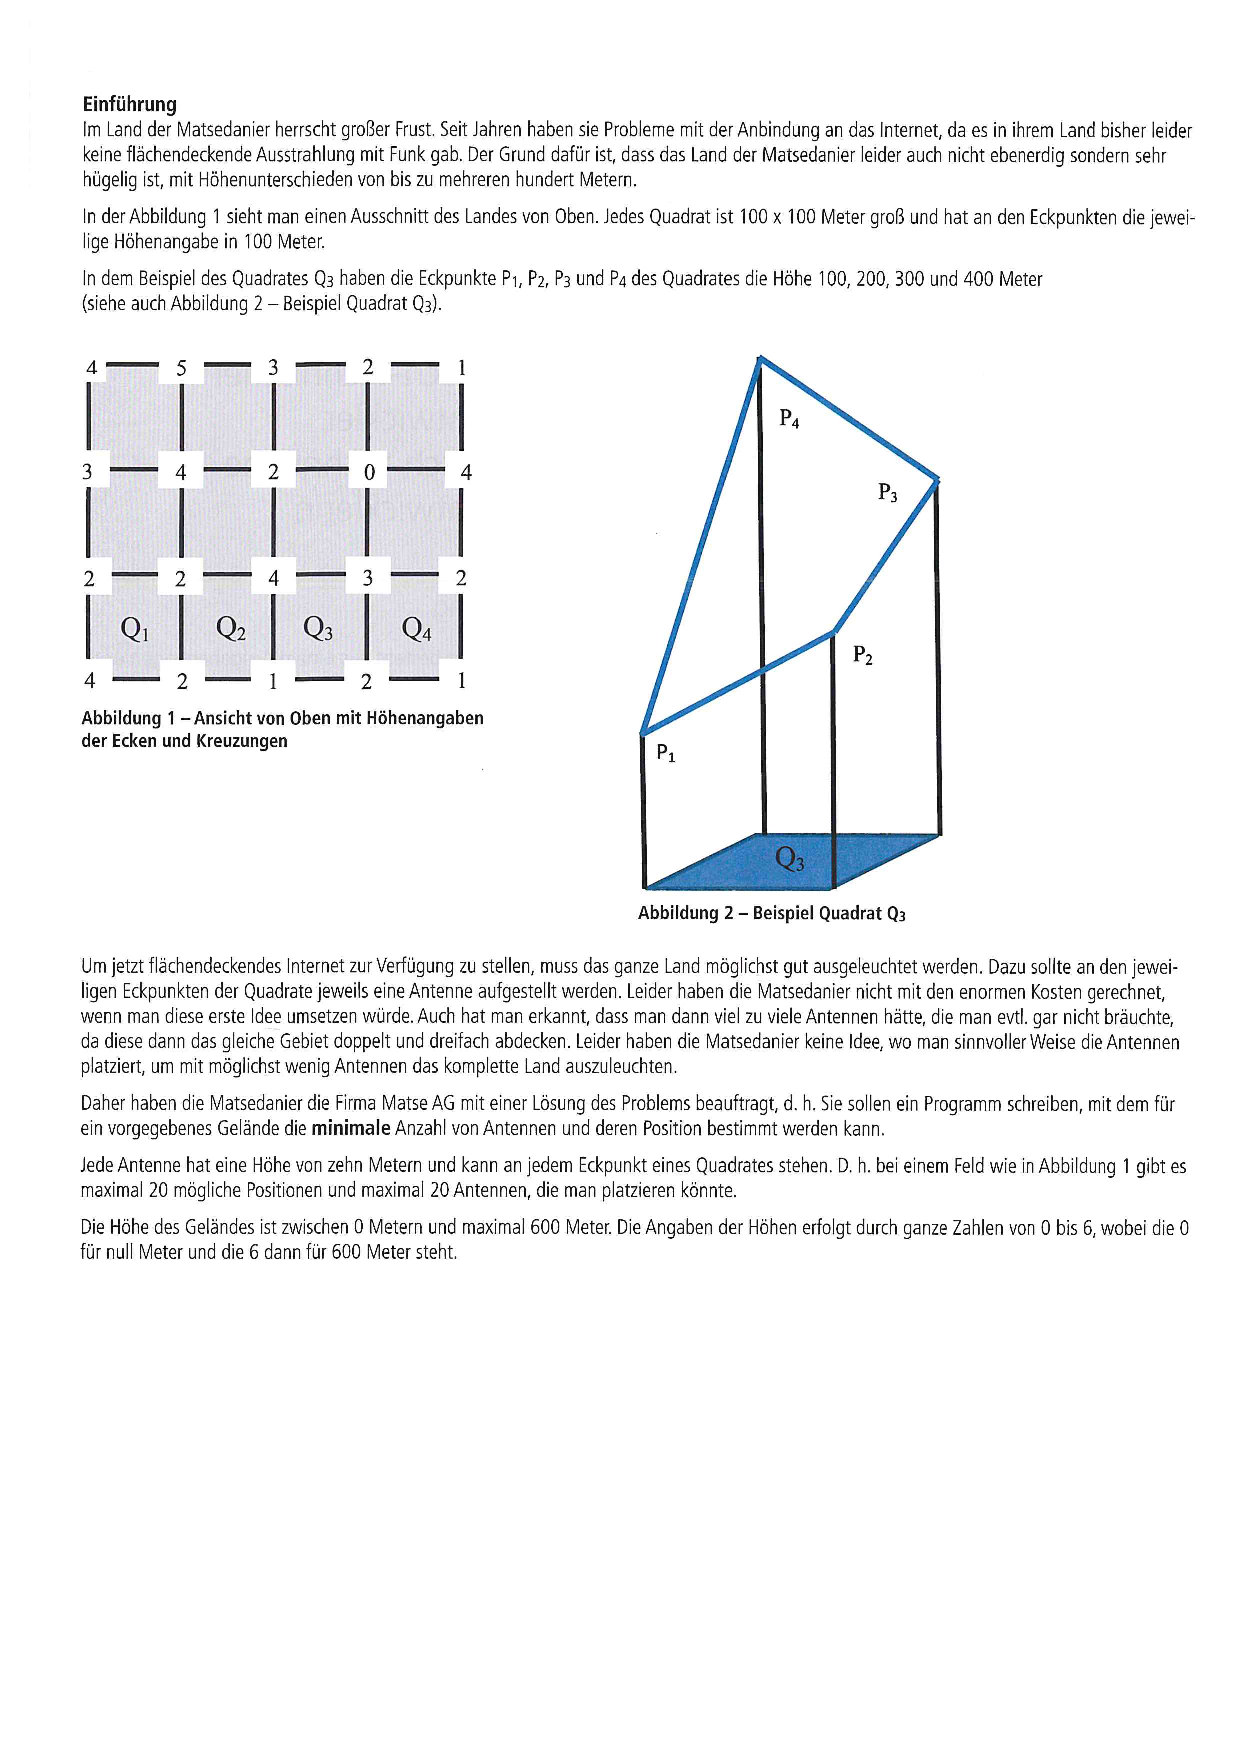
\includepdf[scale=0.8, pages=1,pagecommand=\chapter{Aufgabenstellung}\label{ch:aufgabenstellung}, offset=0 -3cm]{images/Aufgabenstellung}
% \includepdf[pages=2-]{images/Aufgabenstellung}
    \chapter{Quellcode}\label{ch:quellcode}
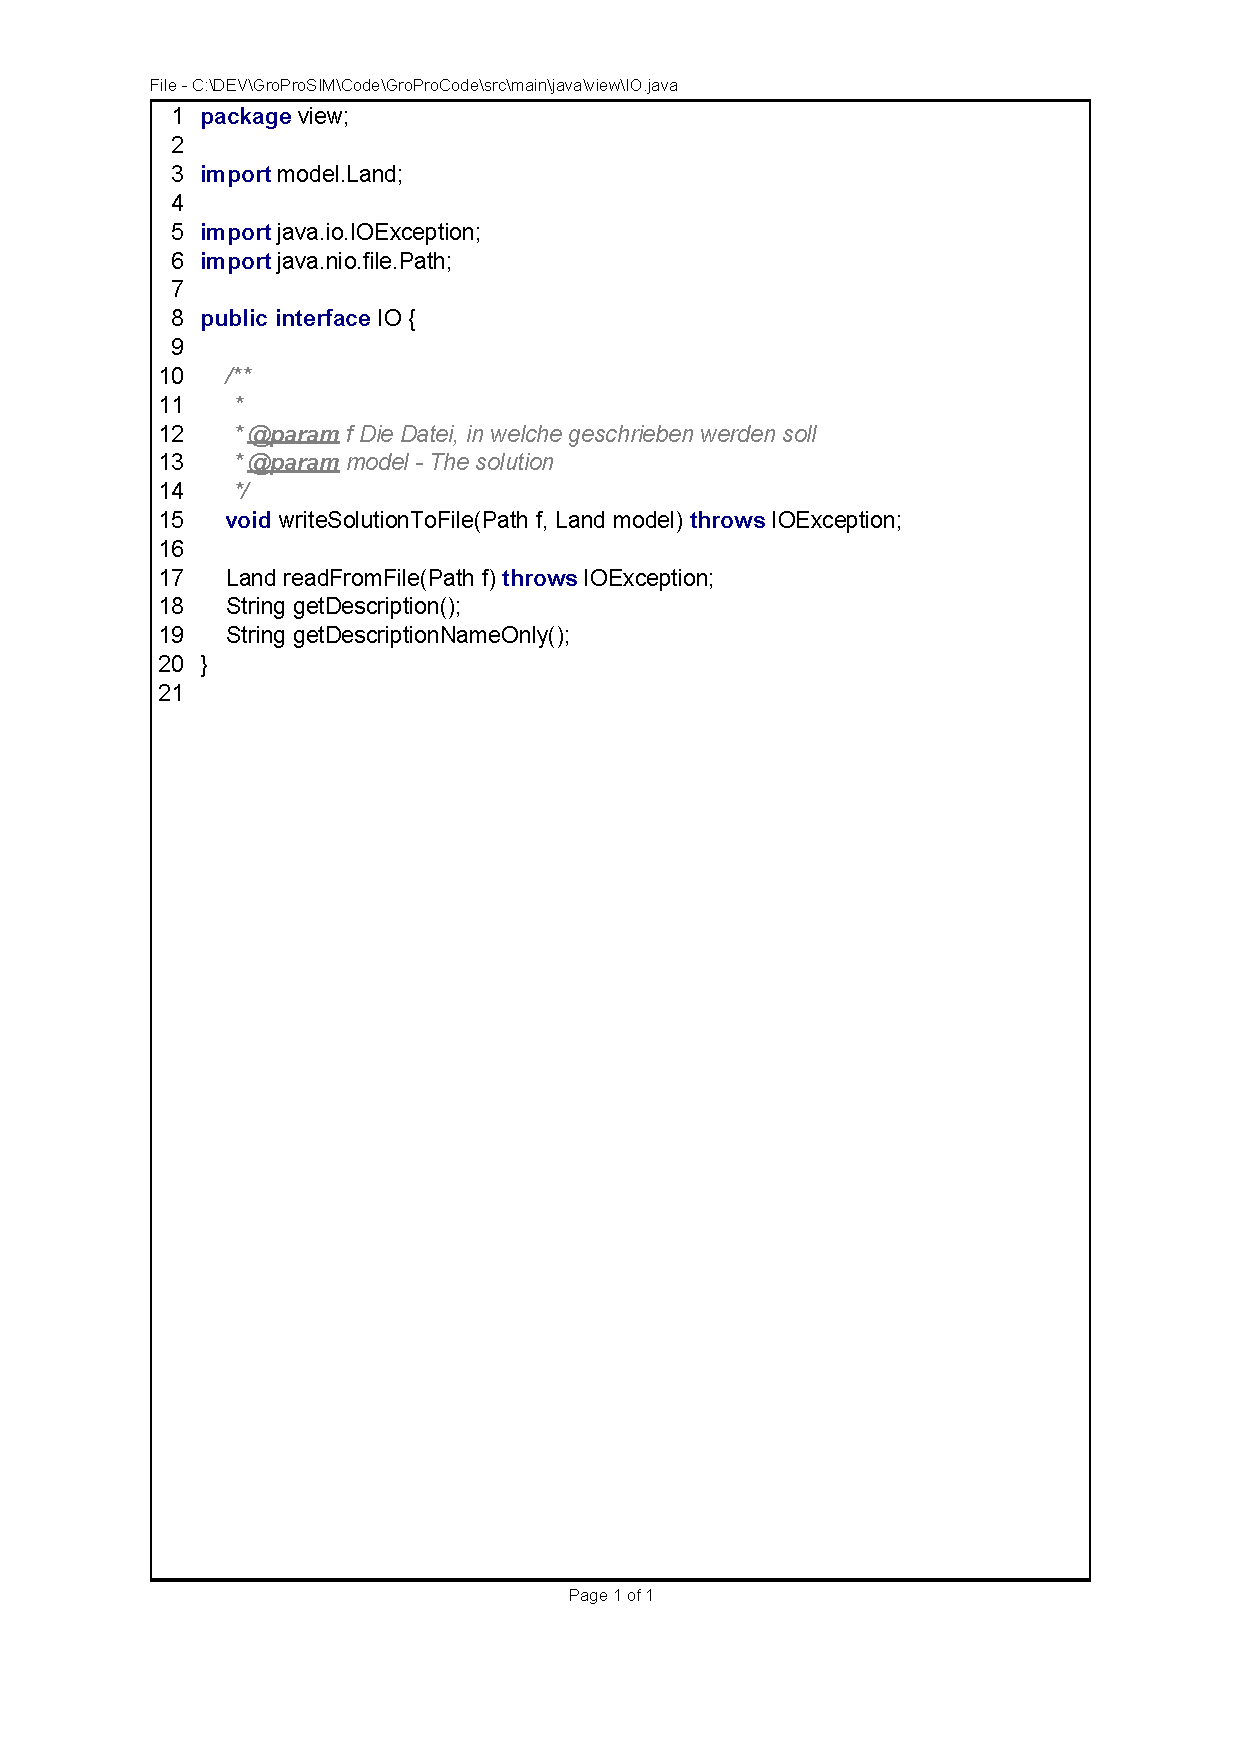
\includepdf[pages=-]{images/SourceCode}
    \include{chapters/H-In-Out-Put-Testdokumentation}
\end{document}